
% Judul dokumen
\title{Buku Tugas Akhir ITS}
\author{Meliaz, Muhammad Roychan}

% Pengaturan ukuran teks dan bentuk halaman dua sisi
\documentclass[10pt,twoside]{report}

% START CUSTOM
\usepackage{float}
% END CUSTOM

% Pengaturan ukuran halaman dan margin
\usepackage[a5paper,top=25mm,left=25mm,right=20mm,bottom=25mm]{geometry}

% Pengaturan ukuran spasi
\usepackage[singlespacing]{setspace}

% Pengaturan format bahasa
\usepackage[indonesian]{babel}

% Pengaturan detail pada file PDF
\usepackage[pdfauthor={\@author},bookmarksnumbered,pdfborder={0 0 0}]{hyperref}

% Pengaturan jenis karakter
\usepackage[utf8]{inputenc}

% Pengaturan pewarnaan
\usepackage[table,xcdraw]{xcolor}

% Pengaturan kutipan artikel
\usepackage[numbers]{natbib}

% Package lainnya
\usepackage{changepage}
\usepackage{enumitem}
\usepackage{eso-pic}
\usepackage{etoolbox}
\usepackage{graphicx}
\usepackage{lipsum}
\usepackage{lmodern}
\usepackage{longtable}
\usepackage{tabularx}
\usepackage{wrapfig}

% Definisi untuk "Hati ini sengaja dikosongkan"
\patchcmd{\cleardoublepage}{\hbox{}}{
  \thispagestyle{empty}
  \vspace*{\fill}
  \begin{center}\textit{[Halaman ini sengaja dikosongkan]}\end{center}
  \vfill}{}{}

% Pengaturan penomoran halaman
\usepackage{fancyhdr}
\fancyhf{}
\renewcommand{\headrulewidth}{0pt}
\pagestyle{fancy}
\fancyfoot[CE,CO]{\thepage}
\patchcmd{\chapter}{plain}{fancy}{}{}
\patchcmd{\chapter}{empty}{plain}{}{}

% Pengaturan format judul bab
\usepackage{titlesec}
\titleformat{\chapter}[display]{\bfseries\Large}{BAB \centering\Roman{chapter}}{0ex}{\vspace{0ex}\centering}
\titleformat{\section}{\bfseries\large}{\MakeUppercase{\thesection}}{1ex}{\vspace{1ex}}
\titleformat{\subsection}{\bfseries\large}{\MakeUppercase{\thesubsection}}{1ex}{}
\titleformat{\subsubsection}{\bfseries\large}{\MakeUppercase{\thesubsubsection}}{1ex}{}
\titlespacing{\chapter}{0ex}{0ex}{4ex}
\titlespacing{\section}{0ex}{1ex}{0ex}
\titlespacing{\subsection}{0ex}{0.5ex}{0ex}
\titlespacing{\subsubsection}{0ex}{0.5ex}{0ex}

% Pengaturan format potongan kode
\usepackage{listings}
\definecolor{comment}{RGB}{0,128,0}
\definecolor{string}{RGB}{255,0,0}
\definecolor{keyword}{RGB}{0,0,255}
\lstdefinestyle{codestyle}{
  commentstyle=\color{comment},
  stringstyle=\color{string},
  keywordstyle=\color{keyword},
  basicstyle=\footnotesize\ttfamily,
  numbers=left,
  numberstyle=\tiny,
  numbersep=5pt,
  frame=lines,
  breaklines=true,
  prebreak=\raisebox{0ex}[0ex][0ex]{\ensuremath{\hookleftarrow}},
  showstringspaces=false,
  upquote=true,
  tabsize=2,
}
\lstset{style=codestyle}

% Isi keseluruhan dokumen
\begin{document}

  % Sampul luar Bahasa Indonesia
  \newcommand\covercontents{sampul/konten-id.tex}
  \input{sampul/sampul-luar.tex}

  % Atur ulang penomoran halaman
  \setcounter{page}{1}

  % Sampul dalam Bahasa Indonesia
  \renewcommand\covercontents{sampul/konten-id.tex}
  \input{sampul/sampul-dalam.tex}
  \clearpage
  \cleardoublepage

  % Sampul dalam Bahasa Inggris
  \renewcommand\covercontents{sampul/konten-en.tex}
  \input{sampul/sampul-dalam.tex}
  \cleardoublepage

  % Pengaturan ukuran indentasi paragraf
  \setlength{\parindent}{2em}

  % Pengaturan ukuran spasi paragraf
  \setlength{\parskip}{1ex}

  % Pernyataan keaslian
  \begin{center}
  \large
  \textbf{PERNYATAAN KEASLIAN\\TUGAS AKHIR}
\end{center}

% Menyembunyikan nomor halaman
\thispagestyle{empty}

\vspace{2ex}

% Ubah paragraf-paragraf berikut sesuai dengan yang ingin diisi pada pernyataan keaslian

Dengan ini saya menyatakan bahwa isi sebagian maupun keseluruhan Tugas Akhir sada dengan judul \textbf{"Manuver \textit{Autonomous Car }ITS di Bundaran atau \textit{U-Turn }Menggunakan \textit{Deep Reinforcement Learning}"} adalah benar-benar hasil karya intelektual mandiri, diselesaikan tanpa menggunakan bahan-bahan yang tidak diijinkan da bukan karya pihak lain yang saya akui sebagai karya sendiri.

Semua referensi yang dikutip maupun dirujuk telah ditulis secara lengkap pada daftar pustaka.

Apabila ternyata pernyataan ini tidak benar, saya bersedia menerima sanksi sesuai peraturan yang berlaku.

\vspace{4ex}

\begin{flushright}
  \begin{tabular}[b]{c}
    % Ubah kalimat berikut sesuai dengan tempat, bulan, dan tahun penulisan
    Surabaya, Juni 2021\\
    \\
    \\
    \\
    \\
    % Ubah kalimat-kalimat berikut sesuai dengan nama dan NRP mahasiswa
    Muhammad Roychan Meliaz\\
    0721 17 4000 0012
  \end{tabular}
\end{flushright}

  \cleardoublepage

  % Lembar pengesahan
  \begin{center}
	\large
  \textbf{LEMBAR PENGESAHAN}
\end{center}

% Menyembunyikan nomor halaman
\thispagestyle{empty}

\begin{center}
  % Ubah kalimat berikut dengan judul tugas akhir
  \textbf{Manuver Autonomous Car ITS di Bundaran atau U-Turn Menggunakan Deep Reinforcement Learning}
\end{center}

\begingroup
  % Pemilihan font ukuran small
  \small

  \begin{center}
    % Ubah kalimat berikut dengan pernyataan untuk lembar pengesahan
    Tugas Akhir ini disusun untuk memenuhi salah satu syarat memperoleh gelar Sarjana Teknik di Institut Teknologi Sepuluh Nopember Surabaya
  \end{center}

  \begin{center}
    % Ubah kalimat berikut dengan nama dan NRP mahasiswa
    Oleh: Muhammad Roychan Meliaz(NRP. 0721 17 4000 0012)
  \end{center}

  \begin{center}
    % Ubah kalimat-kalimat berikut dengan tanggal ujian dan periode wisuda
    Tanggal Ujian : Juli 2021\\
    Periode Wisuda : September 2021
  \end{center}

  \begin{center}
    Disetujui Oleh:
  \end{center}

  \begingroup
    % Menghilangkan padding
    \setlength{\tabcolsep}{0pt}

    \noindent
    \begin{tabularx}{\textwidth}{X c}
      % Ubah kalimat-kalimat berikut dengan nama dan NIP dosen pembimbing pertama
      Prof. Dr. Ir. Mauridhi Hery Purnomo, M.Eng.          & (Pembimbing I) \\
      NIP: 	19580916 198601 1 001       & ................................... \\
      &  \\
      &  \\
      % Ubah kalimat-kalimat berikut dengan nama dan NIP dosen pembimbing kedua
      Dr. I Ketut Eddy Purnama, ST., MT.     & (Pembimbing II) \\
      NIP: 19690730 199512 1 001        & ................................... \\
      &  \\
      &  \\
      % Ubah kalimat-kalimat berikut dengan nama dan NIP dosen penguji pertama
      %Dr. Galileo Galilei, S.T., M.Sc.  & (Penguji I) \\
      %NIP: 15640215 164201 1 001        & ................................... \\
      &  \\
      &  \\
      % Ubah kalimat-kalimat berikut dengan nama dan NIP dosen penguji kedua
      %Friedrich Nietzsche, S.T., M.Sc.  & (Penguji II) \\
      %NIP: 18441015 190008 1 001        & ................................... \\
      &  \\
      &  \\
      % Ubah kalimat-kalimat berikut dengan nama dan NIP dosen penguji ketiga
      %Alan Turing, ST., MT.             & (Penguji III) \\
      %NIP: 19120623 195406 1 001        & ................................... \\
    \end{tabularx}
  \endgroup

  \vspace{2ex}

  \begin{center}
    % Ubah kalimat berikut dengan jabatan kepala departemen
    Mengetahui, \\
    Kepala Departemen Teknik Komputer FTEIC ITS\\

    \vspace{8ex}

    % Ubah kalimat-kalimat berikut dengan nama dan NIP kepala departemen
    \underline{Dr. Supeno Mardi Susiki Nugroho, ST., MT.} \\
    NIP. 19700313 199512 1 001
  \end{center}
\endgroup

  \cleardoublepage

  % Nomor halaman pembuka dimulai dari sini
  \pagenumbering{roman}

  % Abstrak Bahasa Indonesia
  \begin{center}
  \large\textbf{ABSTRAK}
\end{center}

\addcontentsline{toc}{chapter}{ABSTRAK}

\vspace{2ex}

\begingroup
  % Menghilangkan padding
  \setlength{\tabcolsep}{0pt}

  \noindent
  \begin{tabularx}{\textwidth}{l >{\centering}m{2em} X}
    % Ubah kalimat berikut dengan nama mahasiswa
    Nama Mahasiswa    &:& Muhammad Roychan Meliaz \\

    % Ubah kalimat berikut dengan judul tugas akhir
    Judul Tugas Akhir &:&	Manuver \textit{Autonomous Car} ITS di Bundaran atau \textit{U-Turn} Menggunakan \textit{Deep Reinforcement Learning} \\

    % Ubah kalimat-kalimat berikut dengan nama-nama dosen pembimbing
    Pembimbing        &:& 1. Prof. Dr. Ir. Mauridhi Hery Purnomo, M.Eng. \\
                      & & 2. Dr. I Ketut Eddy Purnama, ST., MT. \\
  \end{tabularx}
\endgroup

% Ubah paragraf berikut dengan abstrak dari tugas akhir
\textit{Autonomus Car }atau kendaraan otonom merupakan kendaraan yang memiliki kemampuan untuk berkendara secara mandiri layaknya dikendalikan manusia dengan mengunakan rangkaian kecerdasan buatan. Pada penelitian ini kami mengajukan riset pengembangan kendaraan otonom iCar ITS (\textit{Intelligent Car }Institut Teknologi Sepuluh Nopember) dengan mengembangkan sistem manuver kendaraan otonom di bundaran atau u-turn dalam lingkungan yang disimulasikan. Dalan lingkungan simulasi, model yang digunakan adalah model kendaraan yang disesuaikan dengan iCar. Pengembangan sistem navigasi dan manuver kendaraan otonom dilakukan menggunakan metode \textit{Deep Reinforcement Learning}, salah satu cabang dari \textit{Machine Learning}. Dari penelitian ini diharapkan dapat dihasilkannya algoritma \textit{reinforcement learning }pada mobil otonom yang mampu melakukan manuver di bundaran atau u-turn dengan efisien.

% Ubah kata-kata berikut dengan kata kunci dari tugas akhir
Kata Kunci: Kendaraan otonom, \textit{Reinforcement Learning}, \textit{Deep Learning}, Simulasi.

  \cleardoublepage

  % Abstrak Bahasa Inggris
  \begin{center}
  \large\textbf{ABSTRACT}
\end{center}

\addcontentsline{toc}{chapter}{ABSTRACT}

\vspace{2ex}

\begingroup
  % Menghilangkan padding
  \setlength{\tabcolsep}{0pt}

  \noindent
  \begin{tabularx}{\textwidth}{l >{\centering}m{3em} X}
    % Ubah kalimat berikut dengan nama mahasiswa
    \emph{Name}     &:& Muhammad Roychan Meliaz \\

    % Ubah kalimat berikut dengan judul tugas akhir dalam Bahasa Inggris
    \emph{Title}    &:& ITS \textit{Autonomous Car} Maneuver at Roundabouts or U-Turn using \textit{Deep Reinforcement Learning} \\

    % Ubah kalimat-kalimat berikut dengan nama-nama dosen pembimbing
    \emph{Advisors} &:& 1. Prof. Dr. Ir. Mauridhi Hery Purnomo, M.Eng. \\
                    & & 2. Dr. I Ketut Eddy Purnama, ST., MT. \\
  \end{tabularx}
\endgroup

% Ubah paragraf berikut dengan abstrak dari tugas akhir dalam Bahasa Inggris
\emph{An autonomous car or autonomous vehicle is a vehicle
	which has the ability to drive independently as if controlled by humans using a series of artificial intelligence. In this study, we propose research on the development of an autonomous vehicle iCar ITS (Intelligent Car Institut Teknologi Sepuluh Nopember) by developing a maneuvering system for autonomous vehicles at roundabouts or u-turns in a simulated environment. In the simulation environment, the model used is a vehicle model adapted to iCar. The development of autonomous vehicle navigation and maneuvering systems is carried out using the Deep Reinforcement Learning method, a branch of Machine Learning. From this research, it is hoped that reinforcement learning algorithms on autonomous cars can be produced that are able to maneuver at roundabouts or u-turns efficiently.}

% Ubah kata-kata berikut dengan kata kunci dari tugas akhir dalam Bahasa Inggris
\emph{Keywords}: \emph{Autonomous Vehicle}, \emph{Reinforcement Learning}, \emph{Deep Learning}, \emph{Simulation}.

  \cleardoublepage

  % Kata pengantar
  \begin{center}
  \Large
  \textbf{KATA PENGANTAR}
\end{center}

\addcontentsline{toc}{chapter}{KATA PENGANTAR}

\vspace{2ex}

% Ubah paragraf-paragraf berikut dengan isi dari kata pengantar

Puji dan syukur kehadirat Allah SWT atas segala limpahan berkah, rahmat, serta ridho-Nya, penulis dapat menyelesaikan penelintian ini dengan judul \textbf{Manuver \textit{Autonomous Car }ITS di Bundaran atau \textit{U-Turn }Menggunakan \textit{Deep Reinforcement Learning}.}

Penelitian ini disusun dalam rangka pemenuhan bidang riset di Departemen Teknik Komputer ITS, sera digunakan sebagai persyaratan menyelesaikan pendidikan Sarjana. Penelitian ini dapat diselesaikan tidak lepas dari bantuan berbagai pihak. Oleh karena itu, penulis mengucapkan terimakasih kepada:

\begin{enumerate}[nolistsep]
	
	\item Keluarga, Ibu, Bapak dan Saudara tercinta yang telah memberikan dorongan baik secara spiritual dan material dalam penyelesaian buku penelitian ini. 
	
\end{enumerate}

\begin{flushright}
  \begin{tabular}[b]{c}
    % Ubah kalimat berikut dengan tempat, bulan, dan tahun penulisan
    Surabaya, Juni 2021\\
    \\
    \\
    \\
    \\
    % Ubah kalimat berikut dengan nama mahasiswa
    Muhammad Roychan Meliaz
  \end{tabular}
\end{flushright}

  \cleardoublepage

  % Daftar isi
  \renewcommand*\contentsname{DAFTAR ISI}
  \setcounter{tocdepth}{4}
  \setcounter{secnumdepth}{4}
  \addcontentsline{toc}{chapter}{\contentsname}
  \tableofcontents
  \cleardoublepage

  % Daftar gambar
  \renewcommand*\listfigurename{DAFTAR GAMBAR}
  \addcontentsline{toc}{chapter}{\listfigurename}
  \listoffigures
  \cleardoublepage

  % Daftar tabel
  \renewcommand*\listtablename{DAFTAR TABEL}
  \addcontentsline{toc}{chapter}{\listtablename}
  \listoftables
  \cleardoublepage

  % Nomor halaman isi dimulai dari sini
  \pagenumbering{arabic}

  % Bab 1 pendahuluan
  \chapter{PENDAHULUAN}
\label{chap:pendahuluan}

% Ubah bagian-bagian berikut dengan isi dari pendahuluan

Penelitian ini di latar belakangi oleh berbagai kondisi yang menjadi acuan. Selain itu juga terdapat beberapa permasalahan yang akan dijawab sebagai luaran dari penelitian.

\section{Latar Belakang}
\label{sec:latarbelakang}

Teknologi kendaraan otonom memiliki sejarah yang cukup panjang. Purwarupa pertama yang dapat berfungsi dengan baik diciptakan pada tahun 1980. Dengan menggunakan kamera, purwarupa ini berhasil menempuh 100km jalan kosong tanpa perlu dikemudikan oleh manusia. Dengan keberhasilan ini, muncul banyak proyek pada tahun 80-an dan 90-an menggunakan sistem serupa yang digunakan untuk menyetir melalui jalan raya, baik pada lalu lintas ringan atau tidak ada sama sekali. Dalam pengembangannya, kendaraan otonom dapat memecahkan masalah keselamatan berkendara dan efisiensinya. Maka dari itu, tujuan utama dilakukan penelitian adalah untuk mencegah atau mengurangi kecelakaan lalu lintas, mengurangi waktu orang berkendara, serta mengurangi emisi karbon.\cite{cit:autonomous_vehicle_future}\par

Salah satu produk \textit{autonomous car }yang tengah dikembangkan adalah iCar ITS (\textit{Intelligent Car }Institut Teknologi Sepuluh Nopember). iCar ITS merupakan purwarupa mobil yang dilengkapi dengan fitur pengemudian secara otonom sebagai hasil riset kolaborasi dari para peneliti ITS dengan berbagai bidang keahlian.\cite{cit:icar_menristekbrin} iCar ITS dioperasikan sebagai mobil komuter yang melayani perjalanan penumpang menuju berbagai tujuan dalam kampus ITS.\cite{cit:icar_its_news}

\iffalse
Salah satu produk kendaraan otonom yang tengah dikembangkan adalah iCar ITS, sebuah mobil yang dilengkapi dengan fitur pengemudian secara otonom yang akan berkeliling di kampus ITS sebagai mobil komuter untuk mengantarkan penumpang menuju berbagai lokasi yang di kehendaki di dalam kampus. Mobil otonom yang dikembangkan oleh ITS dengan nama iCar ITS (Intelligent Car ITS) merupakan purwarupa mobil otonom hasil kolaborasi dari peneliti-peneliti di ITS dari berbagai bidang keahlian. iCar ITS dioperasikan sebagai mobil komuter yang melayani perjalanan dalam kampus ITS.\par
\fi

Metode yang lazim digunakan untuk mengembangkan kendaraan otonom adalah \textit{reinforcement learning}, sebuah bagian dari \textit{machine learning }yang juga merupakan bagian dari \textit{artificial intelligence}. \textit{Reinforcement Learning }adalah sebuah metode pembelajaran mengenai apa yang mesti dilakukan (mengimplementasikan aksi kedalam situasi) pada sebuah masalah/\textit{problem }untuk mendapatkan hasil/\textit{reward }yang maksimal. \textit{Agent }tidak diberi \textit{clue }mengenai aksi apa yang harus dilakukan. \textit{Agent }akan mempelajari aksi dengan prinsip \textit{Trial and Error}, lalu mengambil keputusan berdasarkan \textit{reward }yang didapatkan (\textit{reward }maksimal).

Dalam pengaplikasiannya, iCar ITS masih menggunakan metode tradisional rule-based tanpa memanfaatkan metode \textit{machine learning}. Metode tersebut tidak cukup baik karena pengembang harus memprogram secara manual setiap skenario yang akan dihadapi oleh iCar. Metode tersebut tidak akan bertahan lama mengingat banyaknya skenario dunia nyata yang hampir tidak mungkin untuk diberi solusi secara manual.

\section{Permasalahan}
\label{sec:permasalahan}

Dari pemaparan diatas, didapatkan sebuah rumusan masalah. \textit{Autonomous car }ITS masih belum bisa melakukan manuver di bundaran atau u-turn dengan baik. Diperlukan pendekatan \textit{reinforcement learning }yang memadai agar kendaraan tersebut dapat mempelajari bagaimana caranya melakukan manuver yang lebih baik.
	


\section{Tujuan}
\label{sec:Tujuan}

Dari pembahasan diatas, kami menarik beberapa tujuan dari dilakukannya penelitian berikut, yaitu:
\begin{enumerate}[nolistsep]
	\item Dihasilkannya algoritma \textit{reinforcement learning }pada mobil otonom yang mampu melakukan manuver di bundaran/u-turn dengan efisien.
	\item Mengetahui fitur-fitur apa saja yang dibutuhkan oleh \textit{autonomus car }agar output maksimal.
	
	\iffalse
	Dapat dicontohkan seperti dimana lokasi dan berapa derajat kemiringan dari sensor pada kendaraan yang sebaiknya diaplikasikan.
	\fi
	
\end{enumerate}


\section{Batasan Masalah}
\label{sec:batasanmasalah}

Batasan-batasan dari penelitian ini adalah:

\begin{enumerate}[nolistsep]
	
	\item Riset dilakukan dalam lingkungan simulasi dan menggunakan hanya satu bundaran. Simulator yang digunakan adalah CARLA Simulator dan map yang digunakan adalah Town03.
	
	\item Dilakukan dalam kondisi terkontrol tanpa hadirnya pejalan kaki dan kendaraan lainnya di sekitar agen.
	
	\item Simulasi yang dilakukan hanya berfokus pada kegiatan manuver mobil memutari bundaran dan u-turn.
	
\end{enumerate}


\section{Sistematika Penulisan}
\label{sec:sistematikapenulisan}

Laporan penelitian Tugas akhir ini tersusun dalam sistematika dan terstruktur sehingga mudah dipahami dan dipelajari oleh pembaca maupun seseorang yang ingin melanjutkan penelitian ini. Alur sistematika penulisan laporan penelitian ini yaitu:

\begin{enumerate}[nolistsep]

  \item \textbf{BAB I Pendahuluan}

  Bab ini berisi uraian tentang latar belakang permasalahan, penegasan dan alasan pemilihan judul, sistematika laporan, tujuan dan metodologi penelitian.

  \vspace{2ex}

  \item \textbf{BAB II Tinjauan Pustaka}

  Pada bab ini berisi tentang uraian secara sistematis teori-teori yang berhubungan dengan permasalahan yang dibahas pada penelitian ini. Teori-teori ini digunakan sebagai dasar dalam penelitian, yaitu \textit{Reinforcement Learning}, mobil otonom, dan simulator CARLA.

  \vspace{2ex}

  \item \textbf{BAB III Desain dan Implementasi Sistem}

  Bab ini berisi tentang penjelasan-penjelasan terkait eksperimen yang akan dilakukan dan langkah-langkah data diolah hingga menghasilkan model \textit{reinforcement}. Guna mendukung eksperimen pada penelitian ini, digunakanlah blok diagram atau \textit{work flow} agar sistem yang akan dibuat dapat terlihat dan mudah dibaca untuk implementasi pada pelaksaan tugas akhir.

  \vspace{2ex}

  \item \textbf{BAB IV Pengujian dan Analisa}

  Bab ini menjelaskan tentang pengujian eksperimen yang dilakukan terhadap data dan analisanya. Beberapa teknik \textit{reward} dan hasilnya akan ditunjukan pada bab ini dan dilakukan analisa terhadap hasil model yang didapat dari hasil mengamati lingkungan yang tersaji.

  \vspace{2ex}

  \item \textbf{BAB V Penutup}

  Bab ini merupakan penutup yang berisi kesimpulan yang diambil dari penelitian yang telah dilakukan. Saran dan kritik yang membangun untuk pengembangkan lebih lanjut juga dituliskan pada bab ini.

\end{enumerate}

  \cleardoublepage

  % Bab 2 tinjauan pustaka
  \chapter{TINJAUAN PUSTAKA}
\label{chap:tinjauanpustaka}

% Ubah bagian-bagian berikut dengan isi dari tinjauan pustaka

Demi mendukung penelitian ini, dibutuhkan beberapa teori penunjang sebagai bahan acuan dan referensi. Dengan demikian penelitian ini menjadi lebih terarah.

%------------------------------------------
\iffalse

% Contoh input gambar
\begin{figure}[ht]
  \centering

  % Ubah dengan nama file gambar dan ukuran yang akan digunakan
  \includegraphics[scale=0.35]{gambar/roketluarangkasa.jpg}

  % Ubah dengan keterangan gambar yang diinginkan
  \caption{Peluncuran roket luar angkasa \emph{Discovery} \citep{roketluarangkasa}.}
  \label{fig:roketluarangkasa}
\end{figure}
\% Contoh pembuatan persamaan
\begin{equation}
  \label{eq:hukumpertamanewton}
  \sum \mathbf{F} = 0\; \Leftrightarrow\; \frac{\mathrm{d} \mathbf{v} }{\mathrm{d}t} = 0.
\end{equation}
\fi
%------------------------------------------

\section{Dasar Teori}
\label{sec:dasarteori}

\subsection{Autonomous Vehicle}

\textit{Autonomous Vehicle} atau kendaraan otonom dapat didefinisikan sebagai kendaraan yang mampu melihat lingkungannya, memutuskan rute apa yang akan digunakan untuk mencapai tujuannya, dan mengendarai dirinya secara mandiri. Dengan kata lain bisa dikatakan kendaraan otonom adalah kendaraan pintar atau robot yang menggunakan berbagai sensor, prosesor komputer, dan basis data untuk mengambil alih beberapa atau semua fungsi mengemudi dari operator manusia. Mobil yang dilengkapi teknologi ini akan memiliki kelebihan tersendiri seperti mengurangi tabrakan, energi konsumsi, dan juga polusi.\cite{cit:autonomous_vehicle_future}

\textit{Society of Automotive Engineers }(SAE) \textit{International }mengeluarkan standar dalam tingkatan dari kemudi	otomatis. Terdapat enam tingkatan dalam standar tersebut. Tingkatan – tingkatan tersebut yaitu:\cite{cit:sae_def}
\begin{figure}[H] 
	\centering
	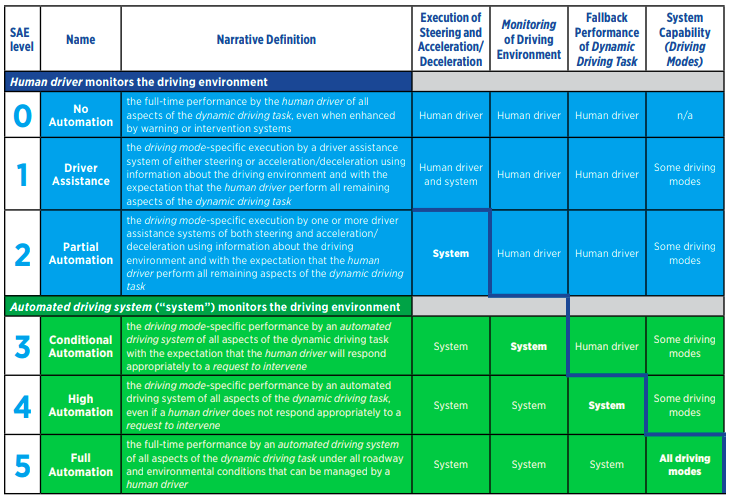
\includegraphics[width=.7\linewidth]{images/autonomous_vehicle_level}
	\caption{Level dari \textit{Autonomous Vehicle }}
	\label{fig:autonomous_vehicle_level}
\end{figure}

\begin{enumerate}[leftmargin=2\parindent]
	\item Level 0, tanpa otomasi. Semua	aspek tugas mengemudi diberikan pada manusia, bahkan ketika ditingkatkan dengan sistem peringatan atau intervensi
	\item Level 1, pendampingan kemudi. Pada tingkat ini fitur-fitur otomasi mulai diterapkan untuk mendukung aspek keselamatan, keamanan, dan kenyamanan pengemudi selama berkendara.
	\iffalse
	\item Level 1, pendampingan kemudi. Adanya bantuan kemudi tertentu oleh sistem kemudi seperti sistem setir atau percepatan/perlambatan dengan menggunakan informasi lingkungan sekitar. Pengemudi manusia melakukan aspek tugas mengemudi yang tersisa.
	\fi
	\item Level 2, otomasi parsial. Kendaraan memiliki minimal 2 fitur otomatis seperti \textit{Steering }dan \textit{Lane Control Assistant }serta \textit{Traffic Jam Assistant}. Sistem mengerem secara otomatis, akselerasi otomatis, dan perlahan–lahan mengambil alih sistem kendali.
	\item Level 3, otomasi kondisional.Kendaraan otonomous level 3 mampu mengemudi sendiri, tetapi hanya dalam kondisi ideal dan dengan keterbatasan. Seorang Pengemudi manusia masih harus mengambil alih jika kondisi jalan berada di bawah kondisi ideal.
	\item Level 4, otomasi tinggi. Kendaraan otonom level 4 dapat mengemudi sendiri tanpa interaksi manusia tetapi akan dibatasi untuk kasus penggunaan yang diketahui. Fitur autonomous Kendaraan level 4 masih dapat dioperasikan hanya pada lingkungan tertentu. 
	\item Level 5, otomasi penuh. Kendaraan berkemampuan level 5 harus dapat memonitor dan bermanuver melalui semua kondisi jalan dan tidak memerlukan intervensi manusia apa pun, menghilangkan kebutuhan akan roda kemudi dan pedal.
\end{enumerate}

Saat ini, level otomasi SAE dari iCar ITS berada pada antara level 3 sampai level 4. \cite{cit:icar_its_news}

\subsection{Machine Learning}

\textit{Machine learning} adalah sebuah cabang dari \textit{artificial intellegence} (AI). \textit{artificial intellegence} memiliki pengertian yang sangat luas, umumnya memiliki arti bagaimana komputer bisa memiliki kecerdasan seperti halnya manusia. \textit{Machine Learning }menurut Arthur Samuel, seorang ilmuwan di bidang komputer yang mencetuskan kecerdasan buatan (\textit{artificial intellegence}) pertama kali, adalah sebuah bidang yang memberi kemampuan komputer untuk belajar tanpa diberi program secara eksplisit. \textit{Machine learning} menggunaan metode statistika untuk membuat komputer dapat mempelajari pola pada data atau biasanya disebut sebagai \textit{pattern recognition}. \cite{cit:ml_patternrecog}

\subsection{Deep Learning}
\begin{figure}[H] 
	\centering
	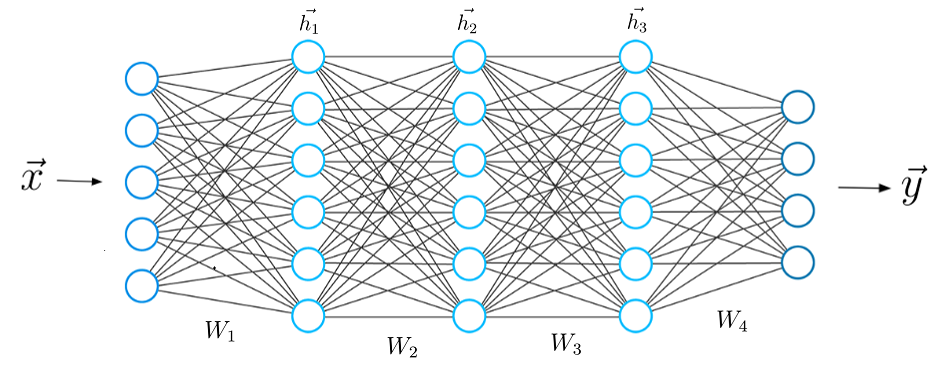
\includegraphics[width=.4\linewidth]{images/deep_learning}
	\caption{Deep Learning}
	\label{fig:deep_learning}
\end{figure}
\textit{Deep learning} merupakan salah satu bagian dari \textit{machine learning}. \textit{Deep learning} dapat dikatakan sebagai algoritma yang menggunakan jaringan syaraf tiruan (\textit{Artificial Neural Network} atau disingkat ANN) untuk menyelesaikan permasalahan pada domain \textit{machine learning}. ANN digunakan sebagai pendekatan dalam pengolahan informasi yang terinspirasi dari bagaimana tiap neuron dalam otak manusia bekerja. Tiap saling berhubungan dan informasi mengalir dari suatu neuron ke neuron lainnya. \cite{cit:deep_learning}

\subsection{Reinforcement Learning}
\begin{figure}[H] 
	\centering
	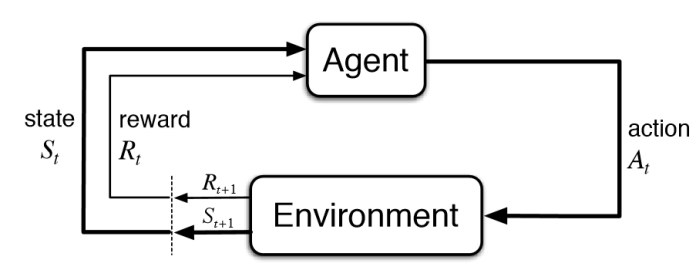
\includegraphics[width=.4\linewidth]{images/reinforcement_learning}
	\caption{Reinforcement Learning}
	\label{fig:reinforcement_learning}
\end{figure}
\textit{Reinforcement Learning }adalah salah satu teknik dari \textit{Machine Learning }dimana \textit{agent }belajar berdasarkan pengalaman yang dialami oleh \textit{agent }tersebut dengan dilengkapi sedikit atau tanpa pengetahuan sebelumnya. \textit{Reinforcement Learning }mempelajari sesuatu hal dengan cara melakukan aksi tertentu dan melihat hasil dari aksi tersebut.\cite{cit:rl_book}

\subsubsection{Skema Kerja Reinforcement Learning}
Seperti pada Gambar \ref{fig:reinforcement_learning}, agen (agent) menerima informasi dari lingkungan (environment) dalam bentuk state. Agen merupakan subjek utama yang melakukan pembelajaran. Lalu, agen memutuskan action apa yang perlu dilakukan berdasarkan informasi lingkungan yang telah didapatkan. Action merupakan serangkaian kemungkinan gerakan yang akan dilakukan oleh agen. Setelah action dilakukan, lingkungan akan berubah dan memberi informasi state baru disertai dengan reward yang didapatkan.

Reward adalah skor yang dapat bernilai positif atau negatif sesuai dengan informasi yang didapatkan dari lingkungan. Agen akan belajar dan melakukan transisi dari state awal hingga state akhir. Proses pembelajaran dari awal hingga akhir ini disebut dengan episode. Sementara state, reward, dan action di tiap perjalanannya dikenal dengan istilah trajectory. Tujuan dari agen adalah untuk memaksimalkan reward yang diperoleh dengan memilih action yang tepat dalam tiap state-nya. Perilaku agen dalam menentukan action yang dipilih berdasarkan state yang diperoleh disebut dengan policy

Salah satu permasalahan yang dihadapi dalam reinforcement learning adalah memodelkan lingkungan yang tepat dalam melakukan pembelajaran terhadap agen. Karena dibutuhkan banyak percobaan yang berulang-ulang untuk dapat memperoleh hasil pembelajaran yang baik, maka perlu dilakukan pembelajaran di Simulator yang tepat sebelum algoritma dapat diimplementasikan di lingkungan sebenarnya.
\iffalse
\subsubsection{Markov Decision Process (MDP)}
\subsubsection{Value Function}
\fi
\subsection{Deep Reinforcement Learning}
\begin{figure}[H] 
	\centering
	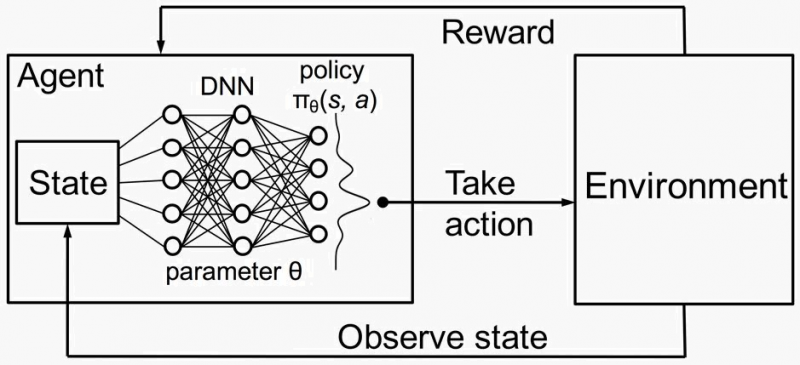
\includegraphics[width=.4\linewidth]{images/deep_rl}
	\caption{Deep Reinforcement Learning}
	\label{fig:deep_reinforcement_learning}
\end{figure}
\textit{Deep Reinforcement Learning }(deep RL) adalah subbidang \textit{machine learning }yang menggabungkan \textit{reinforcement learning }(RL) dan \textit{deep learning}. RL mempertimbangkan masalah pembelajaran agen komputasi untuk membuat keputusan dengan trial and error. Deep RL menggabungkan \textit{deep learning }ke dalam solusinya, memungkinkan agen untuk membuat keputusan dari data masukan yang tidak terstruktur tanpa rekayasa secara manual. Algoritma Deep RL dapat menerima input yang sangat besar dan memutuskan tindakan apa yang harus dilakukan untuk mengoptimalkan tujuan. \textit{Deep Reinforcement Learning }telah digunakan untuk beragam aplikasi termasuk namun tidak terbatas pada robotika, video game, pemrosesan bahasa alami, visi komputer, pendidikan, transportasi, keuangan, dan perawatan kesehatan.\cite{cit:intro_to_deeprl}

\subsection{Convolution Neural Network}
Hubel dan Wiesel merupakan salah satu pelopor pemodelan arsitektur multi-layer perceptron (MLP) yang menjadi dasar dari pengembangan algoritma CNN [12]. MLP merupakan sebuah arsitektur yang memodelkan sebuah sistem jaringan saraf dalam beberapa lapisan neuron, mulai dari yang sederhana hingga kompleks. MLP biasa terdiri dari satu lapisan masukan (input layer), satu atau lebih lapisan tersembunyi (hidden layer), dan satu lapisan keluaran (output layer). MLP yang memiliki banyak lapisan tersembunyi disebut juga Deep Neural Network (DNN).

Untuk menghasilkan performa jaringan arsitektur MLP yang baik, diperlukan metode yang tepat untuk melatih jaringan arsitektur MLP tersebut. Salah satu metode yang dapat digunakan adalah teknik propagasi balik (back-propagation). Propagasi balik merupakan teknik yang memungkinkan MLP untuk belajar dari hasil umpan balik prediksi yang telah dilakukan.

Convolutional neural network (CNN) merupakan salah satu metode pengembangan dari MLP yang banyak digunakan untuk mengenali sebuah pola, seperti pengolahan gambar dan pengenalan suara. Pada tahun 1998, dengan mengimplementasikan feature extraction, Yann Lecun berhasil menjadi yang pertama dalam mengembangkan algoritma CNN, LeNet-5, yang digunakan untuk mengenali tulisan tangan [Need citation].

Arsitektur CNN dibagi menjadi 2 bagian besar, yaitu feature learning dan classification, seperti pada Gambar [need reference] feature learning merupakan lapisan yang berguna menerjemahkan informasi yang terdapat dalam sebuah gambar sebagai sebuah atribut gambar dalam bentuk array multidimensi. Sedangkan classification berguna mengolah array multidimensi tersebut hingga diklasifikasikan dalam fully connected layer.

\subsubsection{Convolution Layer}
Convolutional layer merupakan lapisan yang berguna mengenali objek berdasarkan atribut-atribut yang memiliki lebih banyak informasi. Atribut-atribut yang lebih rendah dapat membentuk atribut yang lebih tinggi, contohnya wajah yang terbentuk dari mata, telinga, hidung, dll. Kemudian, mata yang terbentuk dari lengkungan, bintik hitam, dll.

Untuk dapat mengenali atribut yang terdapat pada sebuah gambar, lapisan konvolusi memerlukan sebuah filter. Filter sendiri merupakan sebuah matriks berukuran 3x3 yang diberi bobot tertentu sesuai dengan jenisnya. Filter sendiri terdiri dari beberapa macam, yaitu filter Mean, Gaussian, atau Median.

Setelah filter ditentukan, maka selanjutnya proses konvolusi dapat dilakukan. Konvolusi merupakan sebuah proses pengaplikasian filter pada sebuah gambar dimana filter digeser secara vertikal dan horizontal pada gambar.

\subsubsection{Pooling Layer}
Pooling layer merupakan lapisan yang bertujuan mengurangi dimensi atau resolusi sebuah gambar dengan tetap mempertahankan informasi yang diperoleh dari gambar. Terdapat 2 jenis pooling yang umum digunakan, yaitu max pooling dan average pooling. Metode max pooling mengambil nilai terbesar dari tiap matriks yang mengalami proses reduksi. Sedangkan average pooling menggunakan nilai rata-rata dalam melakukan proses reduksi matriks. Berikut adalah ilustrasi perbandingan kedua metode tersebut. [NEED IMAGE]

\subsubsection{Fully Connected Layer}
Pada fully connected layer tiap komponen lapisan dalam jaringan akan saling terhubung dengan lapisan lainnya. Penerapan dari fully connected layer sama dengan multi layer perceptron (MLP) yang memiliki tujuan untuk mentransformasikan dimensi data agar proses klasifikasi data dapat dilakukan secara linear. Sebelum data masuk ke fully connected layer, data terlebih dahulu ditransformasi menjadi data satu dimensi agar tidak kehilangan informasi dari tiap neuronnya.

\subsubsection{Padding}
Padding adalah parameter (piksel bernilai 0) yang ditambahkan di setiap sisi gambar untuk mengatasi hilangnya informasi pada gambar saat proses konvolusi berlangsung. Dengan menggunakan padding, dimensi dari keluaran akan tetap sama atau setidaknya tidak berkurang secara signifikan. Contoh aplikasi penggunaan padding dapat dilihat pada Gambar [need reference]. dapat diasumsikan N = 7, F = 3, dan Stride = 1 maka keluaran akan menjadi 5x5 namun karna adanya penambahan satu padding maka keluaran akan tetap berukuran 7x7, yang sama seperti aktualnya.

\subsubsection{Stride}
Stride adalah parameter yang menentukan berapa kali jumlah pergeseran filter dilakukan. Semakin kecil nilai stride yang ditentukan, maka semakin jelas pula informasi yang akan kita dapatkan dari sebuah gambar, namun juga akan membutuhkan proses komputasi yang lebih lama dan besar. Sebagai contoh, diasumsikan sebuah ilustrasi pada Gambar [Need reference] gambar memiliki dimensi ukuran 7x7 dengan menggunakan stride 1. Akan didapatkan keluaran dengan ukuran dimensi 5x5 dan ketika digunakan stride 2 maka keluaran yang didapatkan memiliki ukuran dimensi 3x3. Didapatkan persamaan seperti dalam Persamaan [need reference] dengan N merupakan ukuran masukan, F merupakan ukuran filter, S merupakan ukuran stride, dan O merupakan ukuran keluaran.
\begin{equation}
	\label{eq:stride}
	O = 1 +\frac{N-F}{S}
\end{equation}

\subsubsection{Activation Function}
Fungsi aktivasi merupakan fungsi yang memetakan berbagai masukan dalam suatu neuron menjadi nilai keluaran dari jaringan tersebut. Fungsi aktivasi berperan membuat model jaringan syaraf yang dihasilkan mampu mengatasi permasalahan non linier. Pada dasarnya, terdapat beberapa macam fungsi aktivasi, seperti sigmoid, Tanh, gaussian, ReLU, dll. Namun, pada tugas akhir ini akan digunakan fungsi aktivasi ReLU dalam algoritma CNN dan DQN. Fungsi aktivasi ReLU merupakan fungsi aktivasi yang mengubah nilai keluaran menjadi nol saat nilai masukannya bernilai negatif.

\subsection{Carla Simulator}
\begin{figure}[H] 
	\centering
	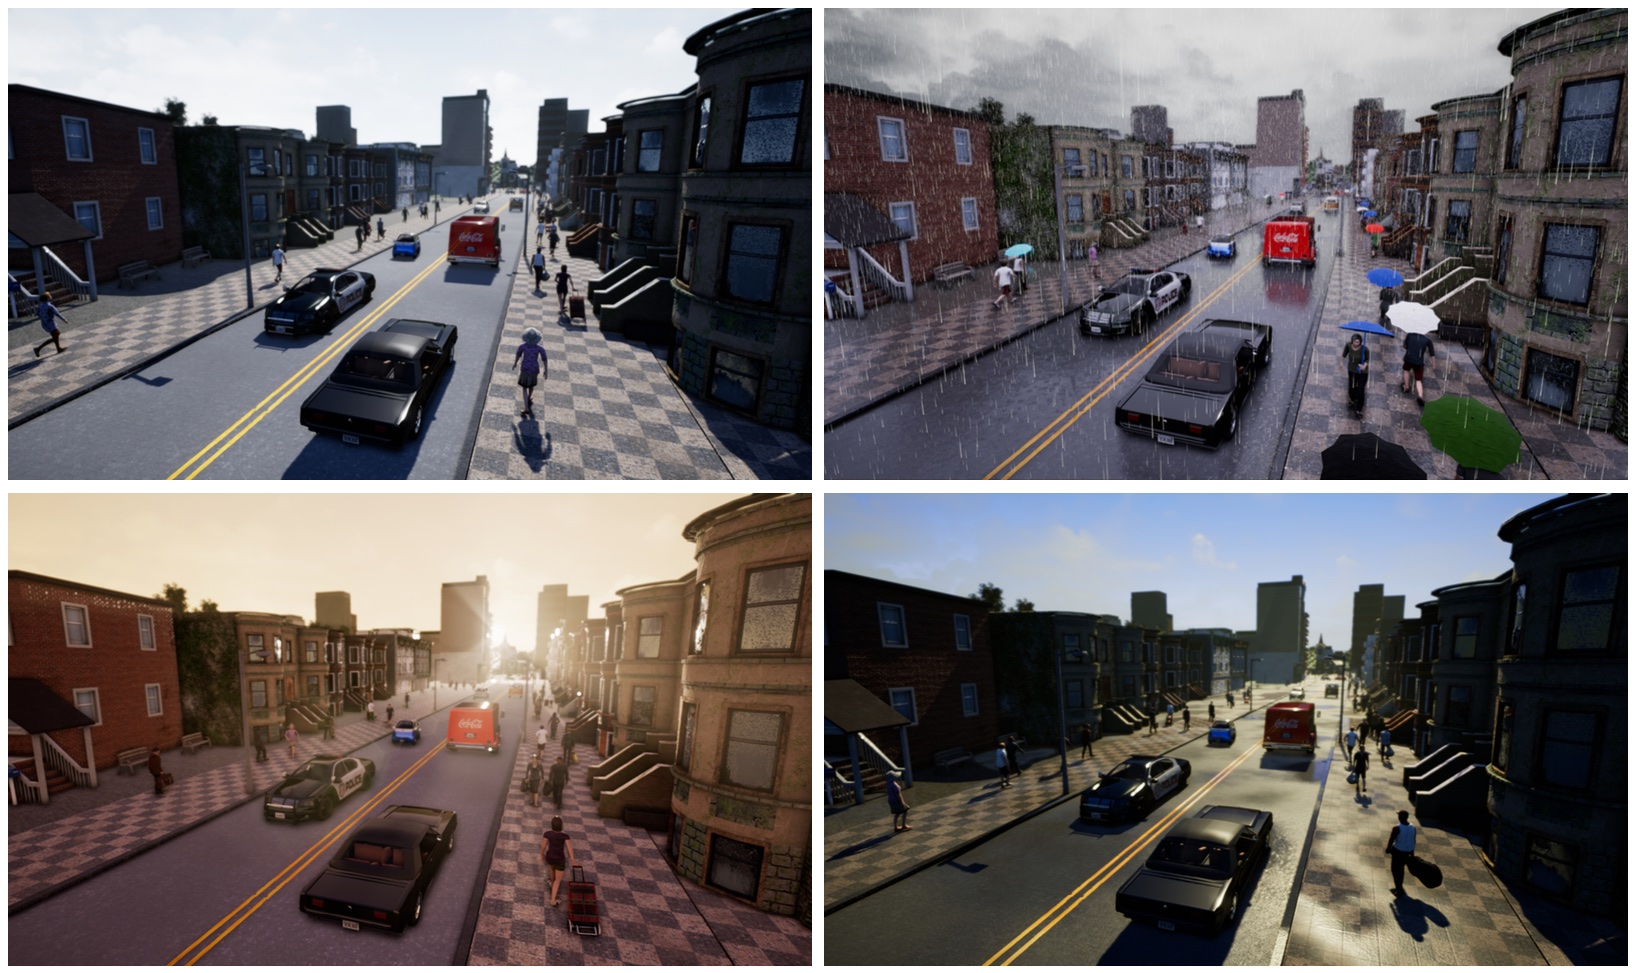
\includegraphics[width=.4\linewidth]{images/carlasim}
	\caption{CARLA Simulator}
	\label{fig:carlasim}
\end{figure}
CARLA merupakan simulator \textit{open source }untuk penelitian kendaraan otonom. CARLA telah dikembangkan untuk mendukung pengembangan pengoperasian, pelatihan, dan validasi sistem pengemudian otonom perkotaan. Dalam tambahan selain kode dan protokol \textit{open source}, CARLA menyediakan aset digital terbuka (tata letak perkotaan, bangunan, kendaraan) dan dapat digunakan secara bebas. Platform simulasi ini mendukung berbagai spesifikasi sensor yang fleksibel serta kondisi lingkungan yang beragam. \cite{cit:carlasim}

%------------------------------------------
\iffalse
\subsection{D4RL}
\begin{figure}[H] 
	\centering
	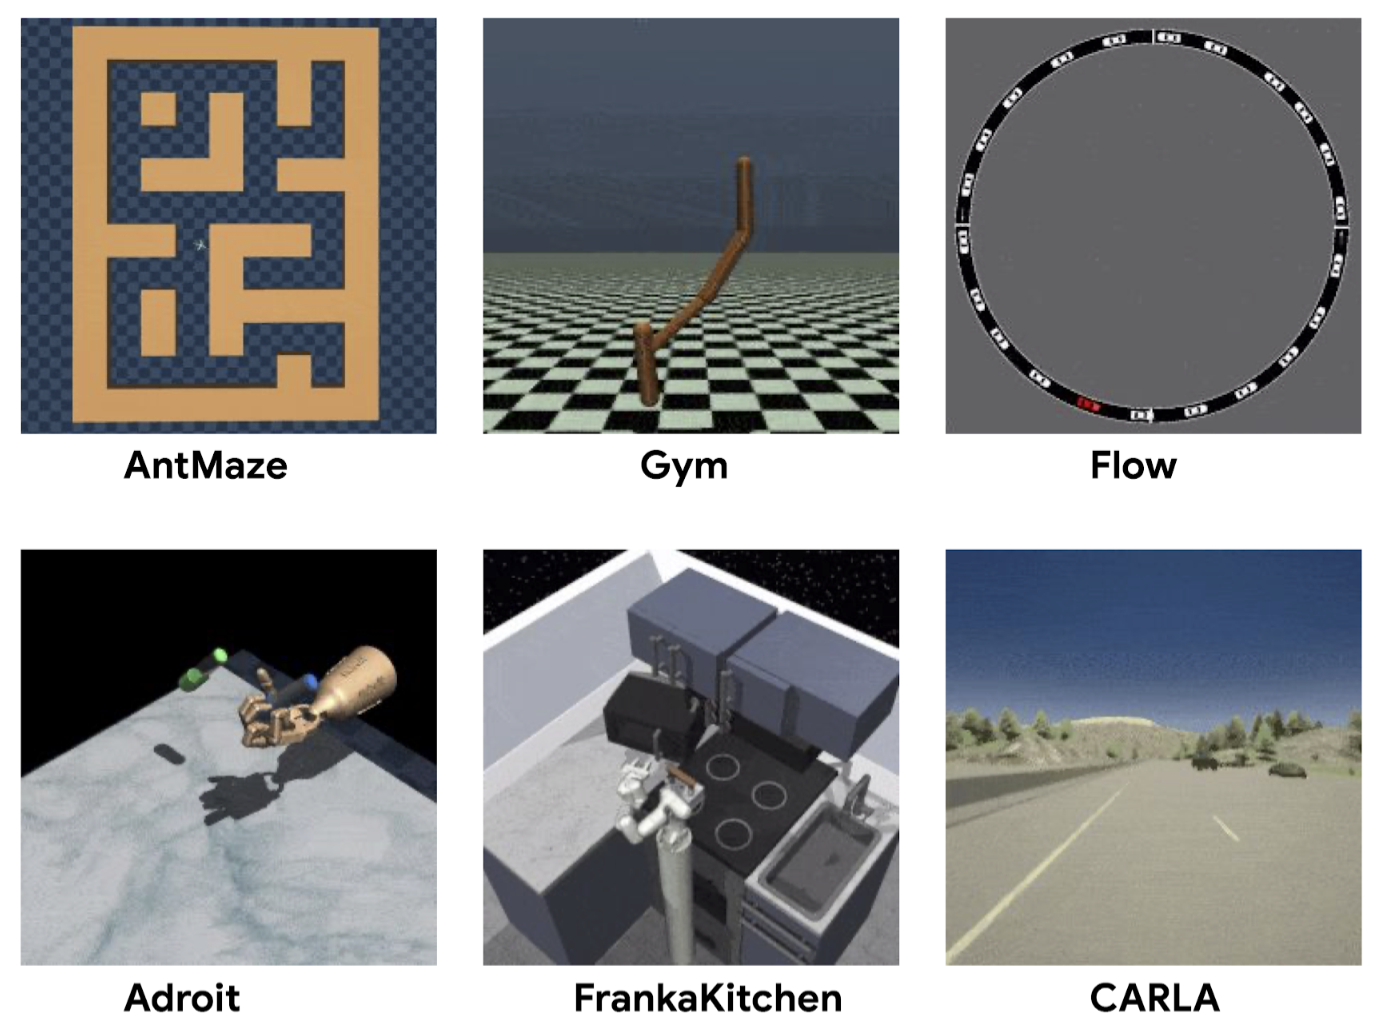
\includegraphics[width=.4\linewidth]{images/d4rl}
	\caption{D4RL: Datasets for Deep Data-Driven Reinforcement Learning \cite{cit:d4rl}}
	\label{fig:d4rl}
\end{figure}
D4RL atau \textit{Datasets for Deep Data-Driven Reinforcement Learning }adalah sebuah \textit{tool benchmark }yang dikhususkan untuk Offline Reinforcement Learning. Diberikan \textit{dataset }dan \textit{task }agar agen dapat melakukan berbagai \textit{task }yang seragam di lingkungan yang sama. \cite{cit:d4rl}
\fi
%------------------------------------------

\section{Penelitian Terkait}
\label{sec:penelitian_terkait}

Beberapa penelitian yang dapat ditemukan terkait dengan topik yang dibawakan oleh tugas akhir ini adalah:
\begin{enumerate}
	\item \textit{Driverless Car: Autonomous Driving Using Deep Reinforcement Learning in Urban Environment oleh A. R. Fayjie, S. Hossain, D. Oualid dan D. Lee (2018)}\newline
	Paper ini menyajikan \textit{deep reinforcement learning }untuk navigasi dan \textit{obstacle avoidance }dari mobil otonom, diaplikasikan dengan \textit{deep Q network }untuk mobil yang disimulasikan di daerah perkotaan. Menggunakan dua tipe sensor sebagai input, yaitu kamera dan laser di depan mobil tersebut. Simulasi yang digunakan diciptakan menggunakan Unity dan mensimulasikan daerah perkotaan dengan jalan 5 lajur.\cite{cit:1}
	
	\item \textit{Controlling an Autonomous Vehicle with Deep Reinforcement Learning oleh A. Folkers, M. Rick dan C. Büskens (2019)}\newline
	Paper ini menyajikan pendekatan kontrol untuk kendaraan otonom menggunakan \textit{deep reinforcement learning}. Melakukan penelitian untuk eksplorasi tempat parkir beserta \textit{obstacle avoidance }untuk kendaraan \textit{full-sized}. Penelitian tersebut merupakan salah satu penelitian pertama yang berhasil menerapkan \textit{deep reinforcement learning }pada kendaraan nyata.\cite{cit:2}
	
	\item \textit{Autonomous Driving in Roundabout Maneuvers Using Reinforcement Learning with Q-Learning}\newline
	Paper ini menyajikan manuver kendaraan otonom di bundaran dengan q-learning menggunakan simulator CARLA.\cite{cit:autonomdrive_roundabout_qlearning} Agent dalam paper tersebut mengambil data kamera rgb serta lidar sebagai parameter dari q-learning.
	
\end{enumerate}

\section{Gap Penelitian}
\label{sec:gap_penelitian}

Dari beberapa penelitian diatas, dapat dilihat ada \textit{gap} penelitian dimana paada penelitian yang dilakukan sebelumnya, belum ada yang melakukan riset mobil otonom untuk melakukan manuver pada bundaran atau u-turn menggunakan \textit{deep reinforcement learning}.

  \cleardoublepage

  % Bab 3 desain dan implementasi
  \chapter{DESAIN DAN IMPLEMENTASI}
\label{chap:desainimplementasi}

% Ubah bagian-bagian berikut dengan isi dari desain dan implementasi
Bab ini akan menjelaskan mengenai sistem perencanaan gerakan mobil otonom, mulai dari konfigurasi sensor pada Simulator mobil otonom, perancangan informasi dan parameter lingkungan berkendara pada simulator mobil otonom, perancangan sistem berkendara mobil otonom, hingga perancangan arsitektur algoritma DQN yang digunakan dalam Tugas Akhir ini.


\section{Deskripsi Sistem}
\label{sec:deskripsisistem}

Sistem pada tugas akhir ini merupakan implementasi dari salah satu disiplin ilmu \textit{Deep Reinforcement Learning} yang berfungsi untuk menciptakan algoritma yang dapat melakukan manuver kendaraan otonom untuk bergerak melewati bundaran atau \textit{u-turn}. Blok diagram metodologi sistem yang digunakan pada penelitian ini dapat dilihat pada Gambar \ref{fig:blockdiagram}.

\section{Persiapan Lingkungan Simulasi}
\label{sec:simulasi}
Menggunakan simulator CARLA, digunakan \textit{map} Town03 CARLA, yang memiliki bundaran dan \textit{u-turn }untuk memfasilitasi pengerjaan tugas akhir. Terdapat dua jenis bundaran yang digunakan pada tugas akhir ini.

\subsection{Bundaran Simpang Empat}
Digunakan bundaran berjumlah simpang empat seperti pada Gambar  \ref{fig:bundaran_town03}. Pada lingkungan ini, \textit{agent} akan \textit{spawn }dari empat titik \textit{spawn} di sekitar bundaran.
\begin{figure}[H] 
	\centering
	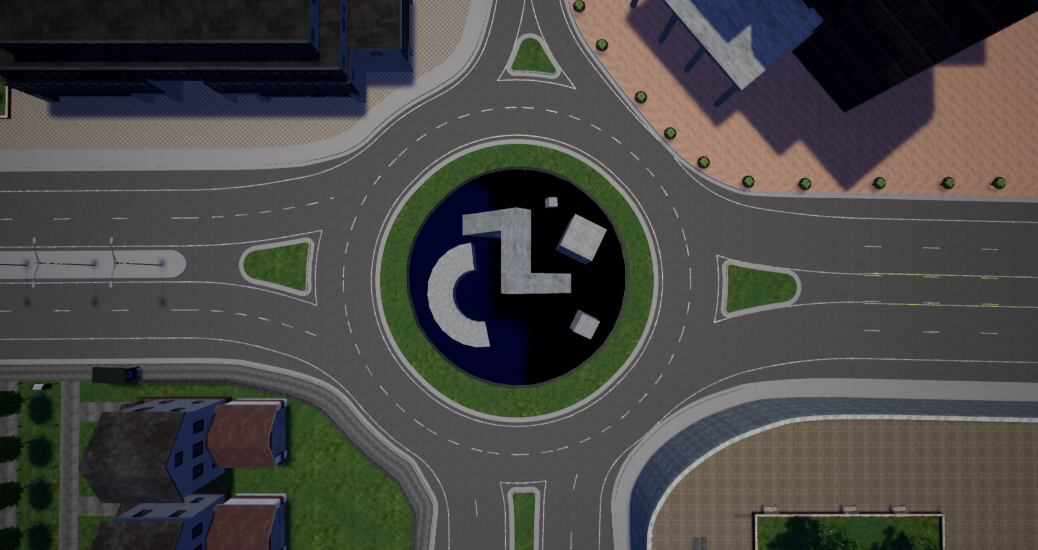
\includegraphics[width=.7\linewidth]{images/bundaran}
	\caption{Bundaran Simpang Empat}
	\label{fig:bundaran_town03}
\end{figure}

\subsection{Bundaran Tanpa Simpang}
Digunakan bundaran tanpa simpang seperti pada Gambar  \ref{fig:bundaran_tanpa_simpang}. Pada lingkungan ini, \textit{agent} akan \textit{spawn }dari sebuah titik \textit{spawn} awal bundaran.
\begin{figure}[H] 
	\centering
	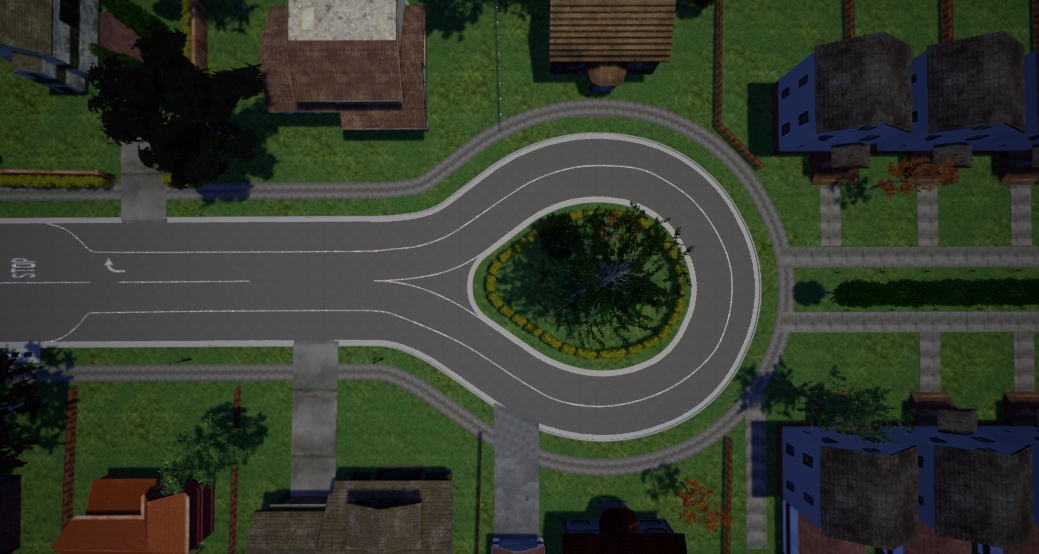
\includegraphics[width=.7\linewidth]{images/bundaran_tanpa_simpang}
	\caption{Bundaran Tanpa Simpang}
	\label{fig:bundaran_tanpa_simpang}
\end{figure}

\section{Sensor}
\label{sec:sensor}
Sensor menggunakan sensor kamera yang diletakkan secara fisik di bagian depan bawah dari agen. Sensor kamera yang digunakan adalah sensor kamera segmentasi. Sensor kamera segmentasi adalah sensor kamera yang memisahkan obyek-obyek di simulator menjadi berbagai warna unik yang solid. Citra yang dihasilkan dari sensor kamera segmentasi pada Gambar \ref{fig:segmentasi} adalah citra lanjutan yang telah di proses dari citra RGB pada gambar \ref{fig:citra_rgb}


\section{Akuisisi Data}
\label{sec:akuisisi_data}
Data citra diambil dari sensor dengan ukuran 480x270. Citra yang digunakan adalah citra segmentasi yang telah disediakan oleh sensor kamera segmentasi dari CARLA Simulator. Terlihat pada Gambar \ref{fig:citra_rgb} merupakan citra awal. Kemudian dilakukan segmentasi pada citra tersebut sehingga setiap obyek dipresentasikan dengan warna solid seperti pada Gambar \ref{fig:segmentasi}

\begin{figure}[H] 
	\centering
	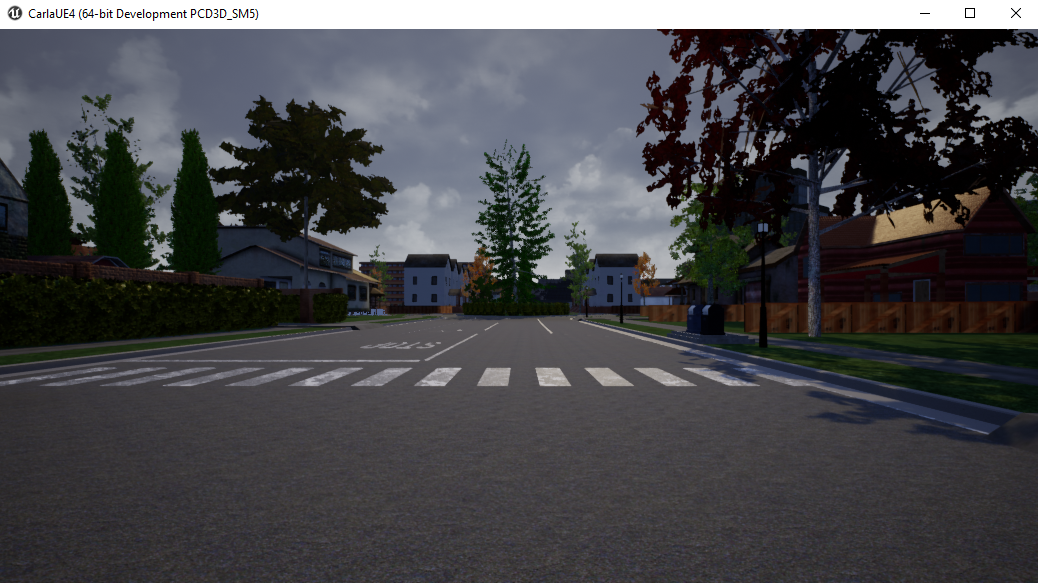
\includegraphics[width=.7\linewidth]{images/rgb}
	\caption{Citra RGB}
	\label{fig:citra_rgb}
\end{figure}
\begin{figure}[H] 
	\centering
	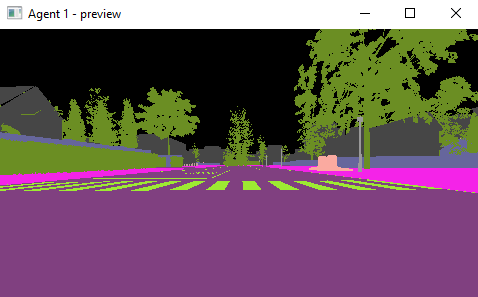
\includegraphics[width=.7\linewidth]{images/segmentasi}
	\caption{Citra Segmentasi}
	\label{fig:segmentasi}
\end{figure}
Ada dua jenis citra yang digunakan dalam tugas akhir ini, yaitu citra segmentasi grayscale dan citra segmentasi lanjutan.

Citra segmentasi grayscale merupakan citra segmentasi yang kemudian diberi filter grayscale agar dapat meminimalkan data yang dianalisa namun tetap mempertahankan fitur yang ada.

\begin{figure}[H] 
	\centering
	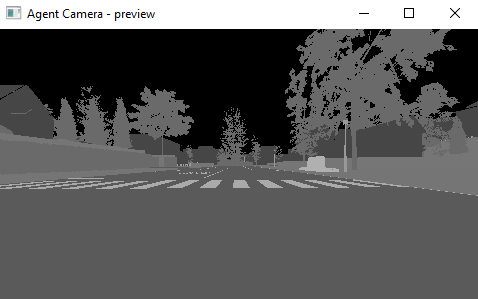
\includegraphics[width=.7\linewidth]{images/grayscale}
	\caption{Citra Segmentasi Grayscale}
	\label{fig:grayscale}
\end{figure}

Citra segmentasi lanjutan merupakan citra segmentasi, yang kemudian di segmentasi kembali menjadi dua jenis obyek, yaitu \textit{drivable }dan \textit{non-drivable}. Obyek \textit{drivable} dipresentasikan dengan warna putih dan obyek \textit{non-drivable} dipresentasikan dengan warna hitam.

\begin{figure}[H] 
	\centering
	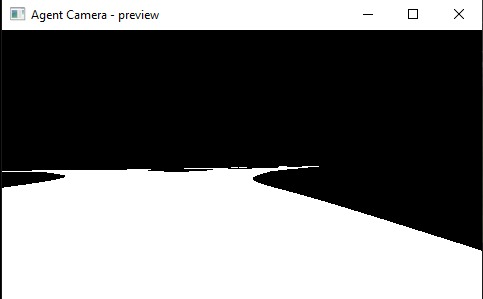
\includegraphics[width=.7\linewidth]{images/segmentasi_hitam_putih}
	\caption{Citra Segmentasi Lanjutan}
	\label{fig:segmentasi_hitam_putih}
\end{figure}

Citra segmentasi grayscale dan citra segmentasi lanjutan akan menjadi hasil akhir akuisi citra yang kemudian akan diberikan ke algoritma DQN untuk melakukan \textit{training} model dan/atau \textit{inference} model.

\section{\textit{Action}}
\label{sec:action}
Ada 3 \textit{action} yang bisa dilakukan oleh \textit{agent}. Diantaranya:

\begin{enumerate}[nolistsep]
	\item \verb=forward=
	
	\textit{Agent} \textit{throttle} dengan nilai 1 dan \textit{steer} dengan nilai 0. Dengan demikian agent akan melakukan gerakan manuver maju.
	
	\item \verb=forward_left=
	
	Agen \textit{throttle} dengan nilai 1 dan \textit{steer} dengan nilai -1. Dengan demikian agent akan melakukan gerakan manuver maju ke depan kiri.

	\item \verb=forward_right=
	
	Agen \textit{throttle} dengan nilai 1 dan \textit{steer} dengan nilai 1. Dengan demikian agent akan melakukan gerakan manuver maju ke depan kanan.
	
\end{enumerate}

\section{\textit{Reward Function}}
\label{sec:sistem_reward}

Fungsi \textit{reward} dirancang agar mobil otonom mampu bergerak sepanjang lintasan dengan cepat dan aman.

\subsection{Bundaran Simpang Empat}Ada empat buah \textit{reward} yang ditetapkan. Masing-masing \textit{reward} memperhatikan referensi \textit{target lane}. \textit{Target lane} adalah garis imajiner yang menjadi target gerakan mobil otonom. Terlihat pada Gambar \ref{fig:target_lane_line}, \textit{target lane} digambarkan dengan titik-titik merah di sekitar bundaran.

\begin{figure}[H] 
	\centering
	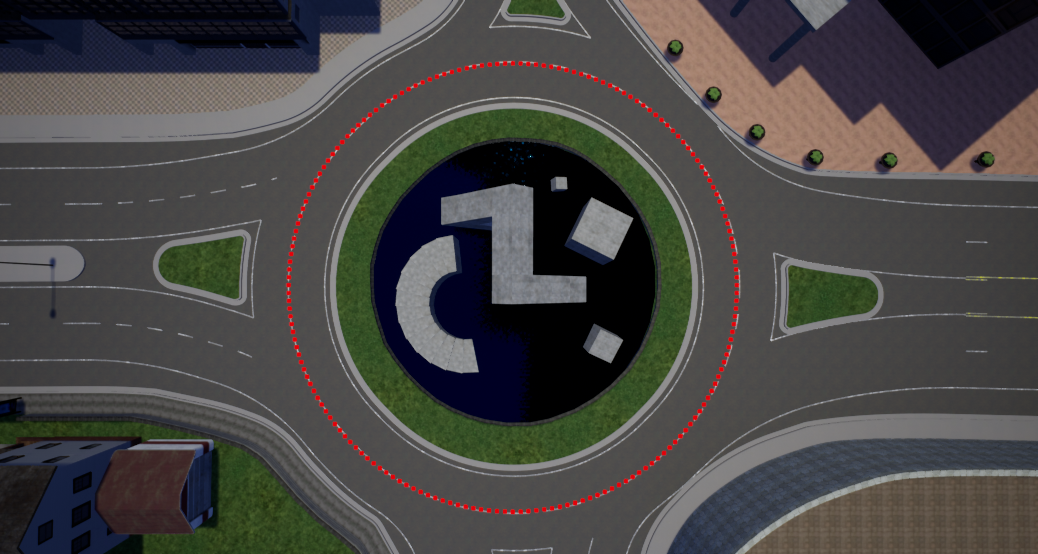
\includegraphics[width=1\linewidth]{images/target_lane_line}
	\caption{\textit{Target lane}}
	\label{fig:target_lane_line}
\end{figure}

\subsubsection{\textit{Reward} 1: Deviasi sudut dari \textit{target lane}}
\textit{Reward }yang digunakan pada \textit{Reward }1 adalah 1/alpha. Alpha adalah sudut \textit{agent }yang menyimpang dari \textit{target lane}. Teknis alpha dijelaskan pada Gambar \ref{fig:reward_anglediff_sketch}. 

\begin{figure}[H] 
	\centering
	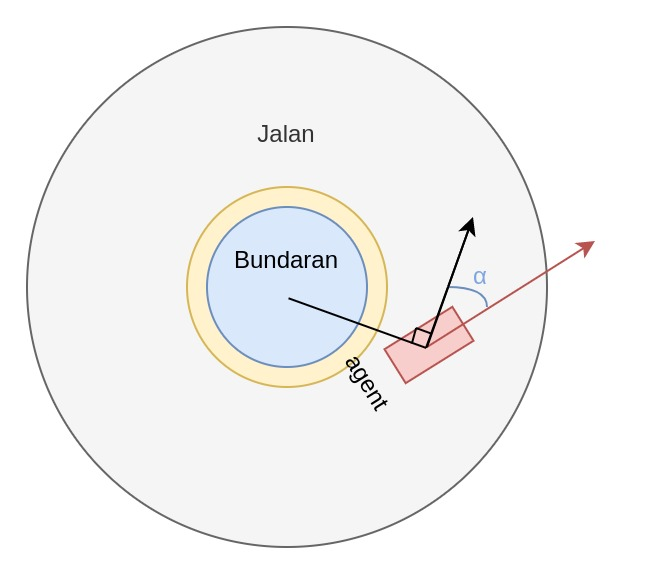
\includegraphics[width=1\linewidth]{images/reward_anglediff_sketch}
	\caption{Reward 1}
	\label{fig:reward_anglediff_sketch}
\end{figure}

Garis hitam merupakan vektor tegak lurus antara titik pusat bundaran ke titik pusat \textit{agent}. Lalu garis merah adalah vektor arah mobil. Dari kedua nilai tersebut, didapat alpha yang merupakan sudut dari kedua vektor tersebut. Kemudian nilai \textit{reward }didefinisikan dengan persamaan \ref{eq:r1}.

\begin{equation}
	R_1 = \frac{1}{\alpha}
	\label{eq:r1}
\end{equation}

Nilai tertinggi \textit{reward} kemudian dibatasi menjadi 1. Hal ini dilakukan agar fluktuasi \textit{reward }yang diberikan ke agent tidak terlalu tinggi untuk perubahan nilai yang kecil, seperti dijelaskan pada persamaan \ref{eq:maxr1}.


\begin{equation}
	R_1 = \begin{cases}R_1 & 0 < R_1 < 1\\1 & R_1 > 1\end{cases}
	\label{eq:maxr1}
\end{equation}

Potongan kode dari fungsi \textit{reward} deviasi sudut terdapat pada Listing \ref{lst:reward_deviasi_sudut}.

\lstinputlisting[
language=Python,
caption={\textit{Reward} Deviasi Sudut.},
label={lst:reward_deviasi_sudut}
]{program/reward_deviasi_sudut.py}

\iffalse
Terlihat pada potongan kode Listing \ref{lst:reward_deviasi_sudut} nilai tertinggi \textit{reward} dibatasi menjadi 1. Hal ini dilakukan agar fluktuasi \textit{reward }yang diberikan ke agent tidak terlalu tinggi untuk perubahan nilai yang kecil.
\fi

\subsubsection{\textit{Reward} 2: Deviasi jarak dari \textit{target lane}}
\textit{Reward} yang digunakan pada \textit{reward} 2 adalah \verb=1/deviasi_jarak*10=. Deviasi jarak adalah jarak terkecil \textit{agent} terhadap \textit{target lane} dalam meter.

\begin{figure}[H] 
	\centering
	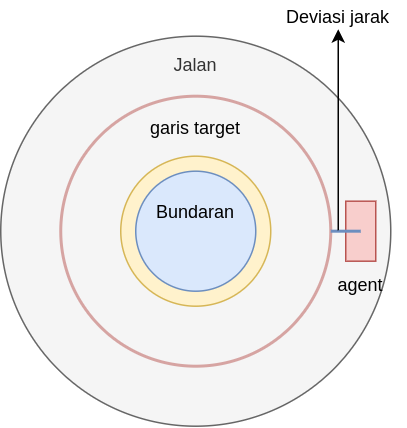
\includegraphics[width=.85\linewidth]{images/reward_deviasi_jarak}
	\caption{Reward 2}
	\label{fig:reward_deviasi_jarak}
\end{figure}

Lingkaran merah merupakan target jalan \textit{agent}. Lalu garis biru adalah jarak dari \textit{agent} menuju target jalan yang kemudian disebut dengan deviasi jarak. Kemudian nilai \textit{reward }didefinisikan dengan persamaan \ref{eq:r2}.

\begin{equation}
	R_2 = \frac{1}{deviasi\_jarak*10}
	\label{eq:r2}
\end{equation}

Nilai tertinggi \textit{reward} kemudian dibatasi menjadi 1. Hal ini dilakukan agar fluktuasi \textit{reward }yang diberikan ke agent tidak terlalu tinggi untuk perubahan nilai yang kecil, seperti dijelaskan pada persamaan \ref{eq:maxr2}.

\begin{equation}
	R_2 = \begin{cases}R_2 & 0 < R_2 < 1\\1 & R_2 > 1\end{cases}
	\label{eq:maxr2}
\end{equation}


Potongan kode dari fungsi \textit{reward} deviasi jarak terdapat pada Listing \ref{lst:reward_deviasi_jarak}.

\lstinputlisting[
language=Python,
caption={\textit{Reward} Deviasi Jarak.},
label={lst:reward_deviasi_jarak}
]{program/reward_deviasi_jarak.py}

\iffalse
Terlihat pula pada potongan kode Listing \ref{lst:reward_deviasi_jarak} nilai tertinggi \textit{reward} dibatasi menjadi 1. Hal ini dilakukan agar fluktuasi \textit{reward} yang diberikan ke \textit{agent} juga tidak terlalu tinggi untuk perubahan nilai yang kecil, seperti pada \textit{Reward} 1.
\fi

Selain \textit{reward} yang bernilai positif, diperlukan juga \textit{reward} yang bernilai negatif untuk mengurangi peluang \textit{agent} melakukan hal yang sebaiknya tidak dilakukan. Ada dua buah \textit{reward} bernilai negatif yang diberikan.

\subsubsection{\textit{Reward} 3: Sentuhan dengan obyek lain}
\textit{Reward} senilai -1 akan diberikan pada \textit{agent} jika \textit{agent} menyentuh obyek lain selain jalan raya, tanah, dan trotoar. Nilai reward didefinisikan pada persamaan \ref{eq:r3}.

\begin{equation}
	R_3 = \begin{cases}-1 & terjadi\: collision\\0 & tidak\:terjadi\: collision\end{cases}
	\label{eq:r3}
\end{equation}


Potongan kode dari fungsi \textit{reward} sentuhan dengan obyek lain terdapat pada Listing \ref{lst:reward_car_collided}.

\lstinputlisting[
language=Python,
caption={\textit{Reward} Sentuhan dengan Obyek Lain.},
label={lst:reward_car_collided}
]{program/reward_car_collided.py}

\subsubsection{\textit{Reward} 4: Deviasi jarak terlalu besar}
\textit{Reward} senilai -0.5 akan diberikan pada \textit{agent} jika jarak antara \textit{agent} dan bundaran lebih besar dari 30 meter. Jarak 30 meter dari bundaran dapat dilihat di Gambar \ref{fig:punishment_lane_line}.

\begin{figure}[H] 
	\centering
	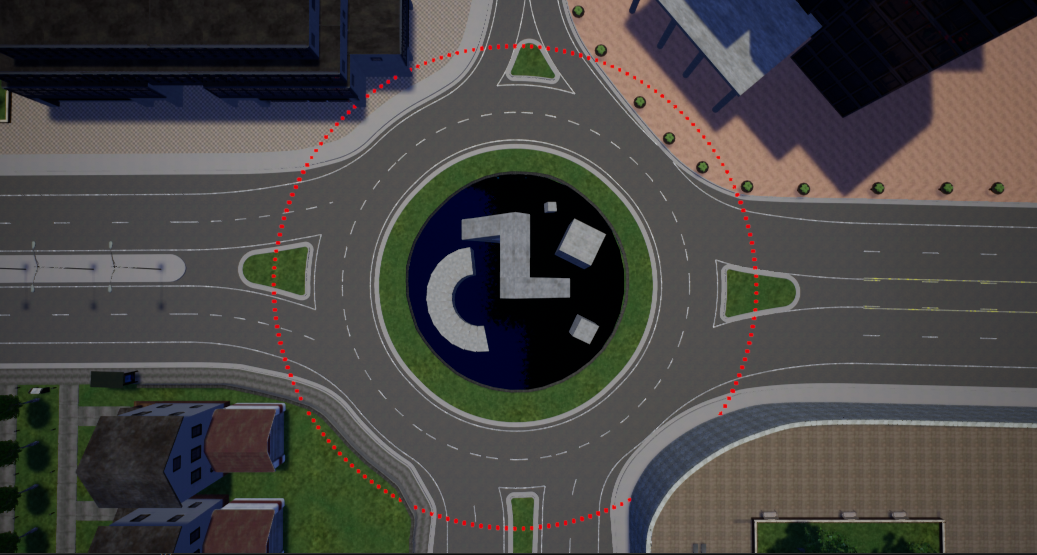
\includegraphics[width=1\linewidth]{images/punishment_lane_line}
	\caption{Batasan jarak}
	\label{fig:punishment_lane_line}
\end{figure}

Nilai reward didefinisikan pada persamaan \ref{eq:r4}.

\begin{equation}
	R_4 = \begin{cases}-0.5 & agent\: keluar\:dari\:lingkaran\:merah\\0 & agent\:di\:dalam\:lingkaran\: merah\end{cases}
	\label{eq:r4}
\end{equation}


Potongan kode dari fungsi \textit{reward} deviasi jarak terlalu besar terdapat pada Listing \ref{lst:reward_too_far}.

\lstinputlisting[
language=Python,
caption={\textit{Reward} Deviasi Jarak Terlalu Besar.},
label={lst:reward_too_far}
]{program/reward_too_far.py}


\subsubsection{\textit{Reward }Total}
Total nilai \textit{reward} didefinisikan dengan jumlah dari seluruh reward seperti yang didefinisikan pada persamaan \ref{eq:rtot}.

\begin{equation}
	R_{total} = R_1+R_2+R_3+R_4
	\label{eq:rtot}
\end{equation}

\subsection{Bundaran Tanpa Simpang}
Pada bundaran tanpa simpang, fungsi \textit{reward} yang diberikan berbeda. Pada kasus ini disediakan titik-titik jalur sebagai \textit{waypoint} yang harus diikuti oleh \textit{agent}.

\begin{figure}[H] 
	\centering
	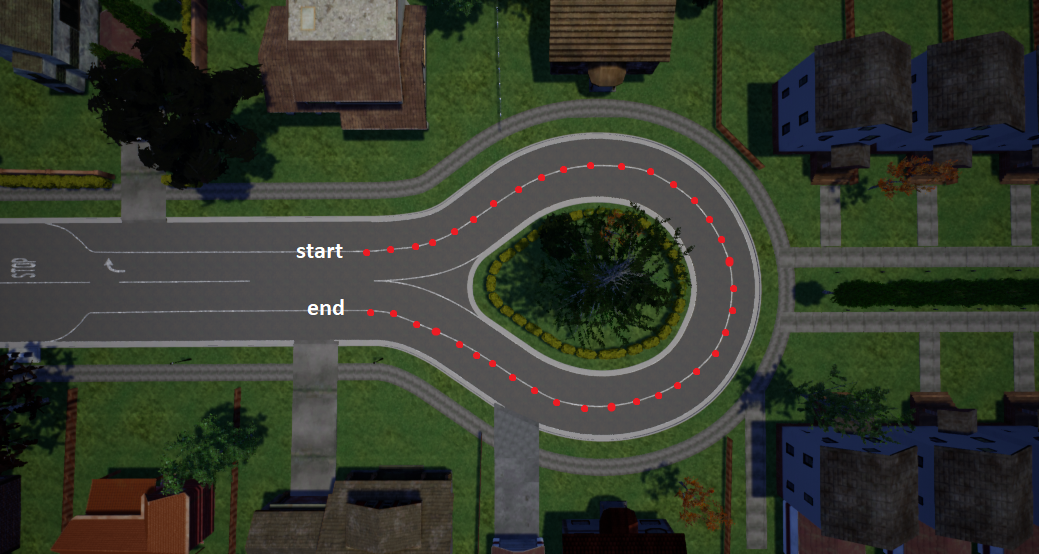
\includegraphics[width=1\linewidth]{images/waypoint}
	\caption{\textit{Waypoint}}
	\label{fig:waypoint}
\end{figure}

\textit{Waypoint} merupakan titik-titik pada \textit{map} sebagai target tujuan jalannya \textit{agent}. Terlihat pada Gambar \ref{fig:waypoint}, titik-titik merah merupakan ilustrasi dari \textit{waypoint}. \textit{Waypoint} berjumlah 100 titik dimana setiap titiknya berjarak satu meter.

\subsubsection{\textit{Reward} 1: Deviasi Sudut dari Waypoint}
\textit{Reward} didefinisikan dengan 1/alpha. Alpha merupakan deviasi sudut arah \textit{agent }terhadap arah titik \textit{waypoint} terdekat dari \textit{agent} + 5.

\begin{figure}[H] 
	\centering
	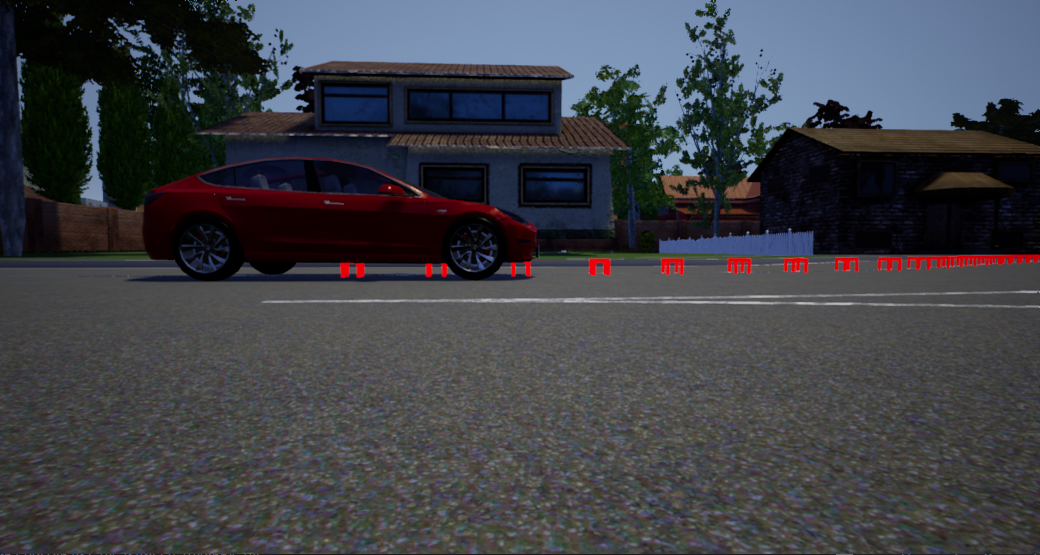
\includegraphics[width=1\linewidth]{images/waypoint_fromside}
	\caption{\textit{Waypoint }dari Sisi \textit{Agent}}
	\label{fig:waypoint_fromside}
\end{figure}

Gambar \ref{fig:waypoint_fromside} menunjukkan bahwa \textit{waypoint} terdekat + 5 dari \textit{agent} berjarak enam meter dari pusat koordinat \textit{agent}.

\begin{figure}[H] 
	\centering
	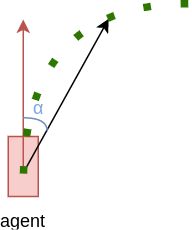
\includegraphics[width=.5\linewidth]{images/reward_alpha}
	\caption{Reward Alpha}
	\label{fig:reward_alpha}
\end{figure}

Ilustrasi fungsi \textit{reward} dapat dilihat pada Gambar \ref{fig:reward_alpha}, dimana titik-titik hijau adalah \textit{waypoints}, garis merah adalah arah dari \textit{agent}, garis hitam adalah arah dari \textit{agent} ke \textit{waypoint}+5 dari \textit{agent}, serta alpha adalah perbedaan sudut dari kedua nilai sudut tersebut. Nilai reward kemudian didefinisikan pada persamaan \ref{eq:r1_nobundaran}.

\begin{equation}
	R_1 = \frac{1}{\alpha}
	\label{eq:r1_nobundaran}
\end{equation}

Nilai tertinggi \textit{reward} kemudian dibatasi menjadi 1. Hal ini dilakukan agar fluktuasi \textit{reward }yang diberikan ke agent tidak terlalu tinggi untuk perubahan nilai yang kecil, seperti dijelaskan pada persamaan \ref{eq:maxr1_nobundaran}.


\begin{equation}
	R_1 = \begin{cases}R_1 & 0 < R_1 < 1\\1 & R_1 > 1\end{cases}
	\label{eq:maxr1_nobundaran}
\end{equation}


Potongan kode dari fungsi \textit{reward} terdapat pada Listing \ref{lst:reward_alpha}.

\lstinputlisting[
language=Python,
caption={\textit{Reward} Alpha.},
label={lst:reward_alpha}
]{program/reward_alpha.py}

\iffalse
Terlihat pula pada potongan kode Listing \ref{lst:reward_alpha} nilai tertinggi \textit{reward} dibatasi menjadi 1. Hal ini dilakukan agar fluktuasi \textit{reward} yang diberikan ke \textit{agent} juga tidak terlalu tinggi untuk perubahan nilai yang kecil, seperti pada \textit{Reward} 1 dan \textit{Reward} 2 pada bundaran simpang empat.
\fi

\subsubsection{\textit{Reward} 2: Sentuhan dengan obyek lain}
\textit{Reward} senilai -1 akan diberikan pada \textit{agent} jika \textit{agent} menyentuh obyek lain selain jalan raya, tanah, dan trotoar. Nilai reward didefinisikan pada persamaan \ref{eq:r2_nobundaran}.

\begin{equation}
	R_2 = \begin{cases}-1 & terjadi\: collision\\0 & tidak\:terjadi\: collision\end{cases}
	\label{eq:r2_nobundaran}
\end{equation}

Potongan kode dari fungsi \textit{reward} sentuhan dengan obyek lain terdapat pada Listing \ref{lst:reward_car_collided}.

\subsubsection{\textit{Reward }Total}
Total nilai \textit{reward} didefinisikan dengan jumlah dari seluruh reward seperti yang didefinisikan pada persamaan \ref{eq:rtot_nobundaran}.

\begin{equation}
	R_{total} = R_1+R_2
	\label{eq:rtot_nobundaran}
\end{equation}

\subsection{End Episode}
\label{sec:end_episode}
Waktu maksimal yang diberikan pada \textit{agent} untuk melakukan proses \textit{training} setiap episodenya adalah 10 detik.

Episode akan berakhir jika waktu maksimal episode berakhir atau agent menyentuh obyek lain selain jalan raya, tanah, dan trotoar.

\section{Parameter DQN}
\label{sec:parameter_dqn}
Penentuan nilai \textit{hyperparameter} yang tepat merupakan salah satu langkah yang penting dilakukan untuk mendapatkan model pembelajaran mesin yang baik. Dalam \textit{machine learning}, \textit{hyperparameter} adalah parameter yang digunakan untuk mengatur jalannya proses pembelajaran mesin. Berbeda dengan parameter model yang nilainya mengalami perubahan seiring berjalannya pembelajaran mesin, \textit{hyperparameter} perlu didefinisikan di awal dan umumnya bernilai tetap sepanjang proses pembelajaran. Dalam tugas akhir ini, \textit{hyperparameter} dari algoritma DQN didefinisikan sebagai berikut:

\subsection{Model}
\label{sec:model}
\begin{table}[H]
	\resizebox{\textwidth}{!}{%
		\begin{tabular}{|l|l|l|}
			\hline
			\textbf{\textit{Hyperparameter}}   & \textbf{Nilai} & \textbf{Deskripsi}                                                                                                                            \\ \hline
			MINIBATCH\_SIZE           & 16             & \begin{tabular}[c]{@{}l@{}}Jumlah sampel pembelajaran yang\\ diproses oleh perhitungan SGD\\ (stochastic gradient) algoritma DQN\end{tabular} \\ \hline
			PREDICTION\_BATCH\_SIZE   & 1              & \begin{tabular}[c]{@{}l@{}}Jumlah sampel yang di prediksi\\ di saat yang bersamaan\end{tabular}                                               \\ \hline
			TRAINING\_BATCH\_SIZE     & 8              & \begin{tabular}[c]{@{}l@{}}Jumlah sampel yang di fit di saat\\ yang bersamaan (lebih besar lebih\\ cepat)\end{tabular}                        \\ \hline
			TRAINER\_MEMORY\_FRACTION & 0.6            &                                                                                                                                               \\ \hline
		\end{tabular}%
	}
\caption{Hyperparameter model.}
\label{tb:hyperparameter_model}
\end{table}

\iffalse
\begin{verbatim}
MINIBATCH_SIZE = 16
PREDICTION_BATCH_SIZE = 1
TRAINING_BATCH_SIZE = MINIBATCH_SIZE // 2
UPDATE_TARGET_EVERY = 100
TRAINER_MEMORY_FRACTION = 0.6
SAVE_CHECKPOINT_EVERY = 50
\end{verbatim}
\fi

\subsection{DQN}
\label{sec:dqn}

\begin{table}[H]
	\resizebox{\textwidth}{!}{%
		\begin{tabular}{|l|l|l|}
			\hline
			\textbf{\textit{Hyperparameter}}   & \textbf{Nilai} & \textbf{Deskripsi}                                                                                                                            \\ \hline
			DISCOUNT                  & 0.99           & \begin{tabular}[c]{@{}l@{}}Nilai faktor \textit{discount }dalam\\ perhitungan \textit{reward }algoritma DQN\end{tabular}                                        \\ \hline
			REPLAY\_MEMORY\_SIZE      & 20\_000        & \begin{tabular}[c]{@{}l@{}}Berapa banyak \textit{step} terakhir yang\\ disimpan untuk \textit{training} model\end{tabular}                                      \\ \hline
			MIN\_REPLAY\_MEMORY\_SIZE & 5\_000         & \begin{tabular}[c]{@{}l@{}}Jumlah \textit{step }minimum dalam\\ memori untuk memulai \textit{training}\end{tabular}                                             \\ \hline
			OPTIMIZER\_LEARNING\_RATE & 0.001          & \begin{tabular}[c]{@{}l@{}}Laju pembelajaran yang digunakan\\ pada \textit{optimizer}\end{tabular}                                                     \\ \hline
			OPTIMIZER\_DECAY          & 0.0            & \begin{tabular}[c]{@{}l@{}}Pengurangan laju pembelajaran\\ pada \textit{optimizer} setiap episodenya\end{tabular}                                      \\ \hline
		\end{tabular}%
	}
	\caption{\textit{Hyperparameter }DQN.}
	\label{tb:hyperparameter_dqn}
\end{table}

\iffalse
\begin{verbatim}
DISCOUNT = 0.99
REPLAY_MEMORY_SIZE = 20_000
MIN_REPLAY_MEMORY_SIZE = 5_000
\end{verbatim}
\fi

\subsection{\textit{Epsilon}}
\label{sec:epsilon}

\begin{table}[H]
	\resizebox{\textwidth}{!}{%
		\begin{tabular}{|l|l|l|}
			\hline
			\textbf{\textit{\textit{Hyperparameter}}}   & \textbf{Nilai} & \textbf{Deskripsi}                                                                                                                            \\ \hline

			START\_EPSILON            & 1              & \begin{tabular}[c]{@{}l@{}}Nilai \textit{epsilon }saat pertamakali\\ mulai \textit{training}\end{tabular}                                                       \\ \hline
			EPSILON\_DECAY            & 0.9995         & \begin{tabular}[c]{@{}l@{}}Penurunan nilai \textit{epsilon} di setiap\\ episodenya\end{tabular}                                                        \\ \hline
			MIN\_EPSILON              & 0.1            & \begin{tabular}[c]{@{}l@{}}\textit{Epsilon }terendah yang\\ diperbolehkan\end{tabular}                                                                 \\ \hline
		\end{tabular}%
	}
	\caption{\textit{Hyperparameter epsilon}.}
	\label{tb:hyperparameter_epsilon}
\end{table}
Penentuan parameter \textit{epsilon} didefinisikan dengan persamaan \ref{eq:eps_decay}.

\begin{equation}
	\epsilon_{episode} = \epsilon_{episode-1} * EPSILON\_DECAY
	\label{eq:eps_decay}
\end{equation}

 \textit{Epsilon} akan bernilai START\_EPSILON (1) saat pertamakali memulai \textit{training }atau pada saat episode 0. Setiap dimulainya episode baru, nilai \textit{epsilon} akan dikali dengan nilai EPSILON\_DECAY (0.9995) hingga pada akhirnya akan bernilai MIN\_EPSILON (0.1) setelah 4700 episode. Pengurangan nilai \textit{epsilon} akan berhenti setelah sampai pada nilai MIN\_EPSILON (0.1), seperti yang didefinisikan pada persamaan \ref{eq:eps_min}.

\begin{equation}
	\epsilon = \begin{cases}\epsilon & MIN\_EPSILON < \epsilon < 1\\MIN\_EPSILON & \epsilon < MIN\_EPSILON\end{cases}	\label{eq:eps_min}
\end{equation}

\iffalse
\begin{figure}[H] 
	\centering
	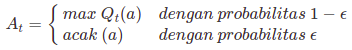
\includegraphics{images/epsilon_formula}
	\caption{Formula Epsilon}
	\label{fig:epsilon_formula}
\end{figure}
\fi

\begin{equation}
	A_t = \begin{cases}max\:Q_t(a) & dengan\:probabilitas\:1-\epsilon\\acak(a) & dengan\:probabilitas\:\epsilon\end{cases}
	\label{eq:at}
\end{equation}

Dari persamaan \ref{eq:at} didapatkan bahwa \textit{action }dari \textit{agent} yang dilakukan pada saat t dipengaruhi oleh epsilon. Saat epsilon tinggi, kemungkinan besar \textit{action} yang dilakukan saat t adalah acak, atau disebut juga dengan eksplorasi. Namun saat epsilon rendah, kemungkinan besar \textit{action} yang dilakukan saat t adalah \textit{action} yang telah diketahui terbaik sesuai kondisi state saat itu, atau disebut juga dengan eksploitasi.

Penentuan parameter \textit{epsilon-greedy} ini dilakukan agar \textit{agent} mampu melakukan kegiatan eksplorasi dan eksploitasi dengan tepat. Sehingga hasil yang didapatkan akan baik dalam waktu cepat.

\iffalse
\begin{verbatim}
START_EPSILON = 1
EPSILON_DECAY = 0.9995
MIN_EPSILON = 0.1
\end{verbatim}
\fi

\section{Arsitektur Model}
\label{sec:arsitektur_model}

Berikut adalah arsitektur yang digunakan:

\begin{table}[H]
	\begin{tabular}{lll}
		\textbf{Layer (type)}                      & \textbf{Output Shape}         & \textbf{Param \#} \\
		conv2d\_1\_input (InputLayer)     & (None, 270, 480, 1)  & 0        \\
		conv2d\_1 (Conv2D)                & (None, 270, 480, 64) & 640      \\
		activation\_1 (Activation)        & (None, 270, 480, 64) & 0        \\
		average\_pooling2d\_1 (AveragePoo & (None, 90, 160, 64)  & 0        \\
		conv2d\_2 (Conv2D)                & (None, 90, 160, 64)  & 36928    \\
		activation\_2 (Activation)        & (None, 90, 160, 64)  & 0        \\
		average\_pooling2d\_2 (AveragePoo & (None, 30, 54, 64)   & 0        \\
		conv2d\_3 (Conv2D)                & (None, 30, 54, 64)   & 36928    \\
		activation\_3 (Activation)        & (None, 30, 54, 64)   & 0        \\
		average\_pooling2d\_3 (AveragePoo & (None, 10, 18, 64)   & 0        \\
		flatten\_1 (Flatten)              & (None, 11520)        & 0        \\
		kmh\_input (InputLayer)           & (None, 1)            & 0        \\
		concatenate\_1 (Concatenate)      & (None, 11521)        & 0        \\
		dense\_1 (Dense)                  & (None, 256)          & 2949632  \\
		dense\_2 (Dense)                  & (None, 3)            & 771     
	\end{tabular}
\caption{Arsitektur model.}
\label{tb:arsitektur_model}
\end{table}

Diberikan konvolusi kepada citra \textit{image} sebanyak 3 kali. Setiap konvolusi dilakukan dengan \textit{average pooling}. Proses selanjutnya setelah konvolusi adalah menambahkan data kecepatan \textit{agent}. Kemudian pada akhir dari proses akan didapatkan \textit{output} \textit{action} berjumlah 3.

Berikut adalah potongan program untuk model 64x3.
\lstinputlisting[
language=Python,
caption={Model 64x3.},
label={lst:bilanganprima}
]{program/model64x3.py}

Berikut adalah potongan program untuk \textit{hidden dense}.
\lstinputlisting[
language=Python,
caption={\textit{Hidden dense}.},
label={lst:bilanganprima}
]{program/hidden_dense.py}


\section{\textit{Training}}
\label{sec:training}

\begin{figure}[H] 
	\centering
	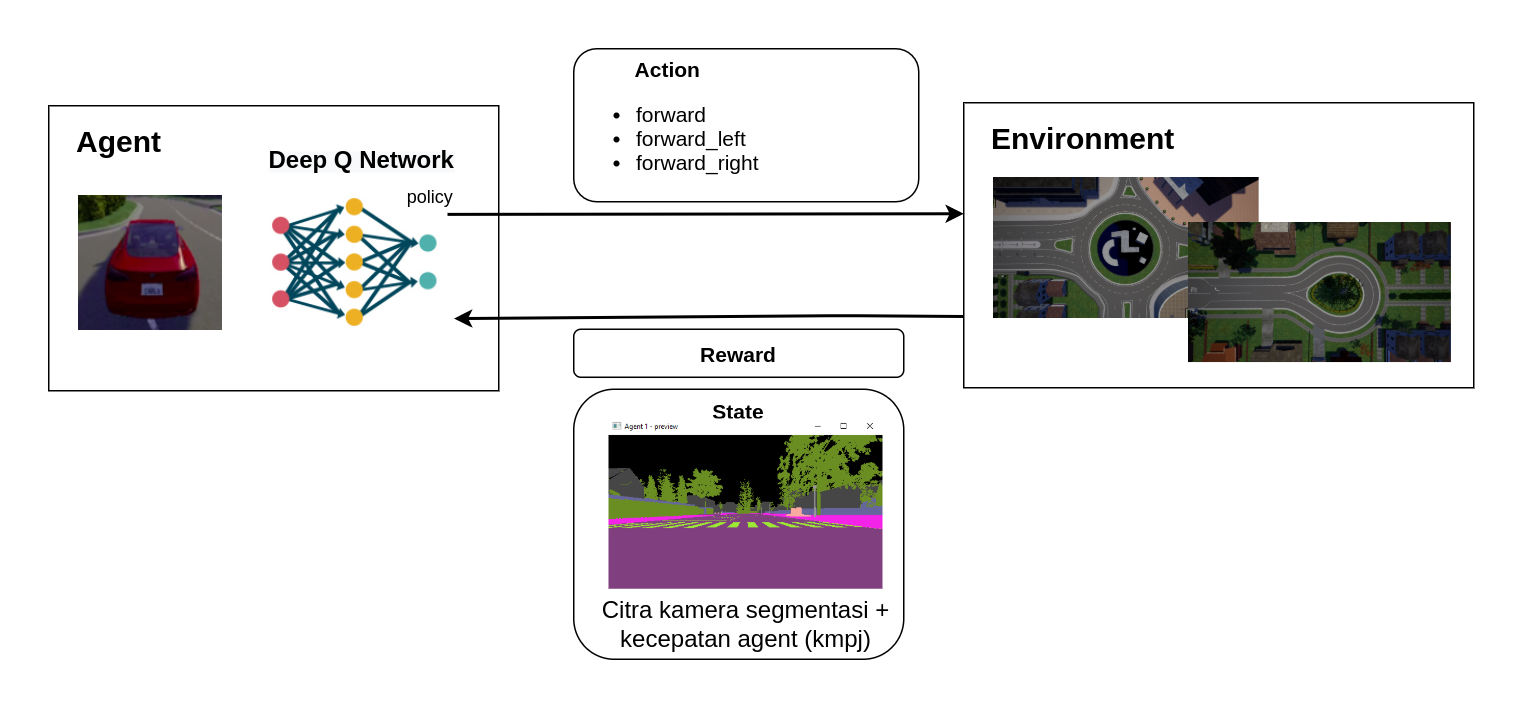
\includegraphics[width=1\linewidth]{images/metodologi}
	\caption{Diagram Blok Metodologi}
	\label{fig:blockdiagram}
\end{figure}

Proses \textit{training} dilakukan setelah seluruh konfigurasi selesai dilakukan. Metodologi \textit{training} dari tugas akhir ini terdapat pada Gambar \ref{fig:blockdiagram}. \textit{Agent} yang berada pada simulasi melakukan suatu \textit{action} yang menyebabkan berubahnya \textit{state}. \textit{State} yang berupa citra segmentasi dan kecepatan \textit{agent} (kmpj) serta \textit{reward }dari \textit{agent} kemudian dikirimkan ke DQN untuk dilakukan \textit{tra}ining. Hasil dari \textit{training} berupa \textit{policy },  akan menentukan\textit{action} yang kemudian akan dilaksanakan oleh \textit{agent}. Kemudian proses tersebut akan terulang kembali menjadi sebuah siklus yang tak henti.

\iffalse
Tugas akhir ini akan menggunakan metode \textit{deep reinforcement learning}, yaitu \textit{reinforcement learning }yang disertai dengan \textit{deep learning }untuk mempelajari \textit{policy }apa yang cocok untuk digunakan oleh \textit{agent}. 

Algoritma \textit{deep reinforcement learning} yang digunakan adalah \textit{Deep Q Network} (DQN). \textit{Deep Q Network} merupakan implementasi \textit{neural network} atau \textit{deep learning} pada \textit{Q-learning}.

Parameter yang diberikan pada DQN adalah citra, serta kecepatan kendaraan dalam nilai kmpj.
\fi





%-----------------------------
%END for C and Python template
\iffalse
% Contoh pembuatan potongan kode
\begin{lstlisting}[
  language=C++,
  caption={Program halo dunia.},
  label={lst:halodunia}
]
#include <iostream>

int main() {
    std::cout << "Halo Dunia!";
    return 0;
}
\end{lstlisting}

% Contoh input potongan kode dari file
\lstinputlisting[
  language=Python,
  caption={Program perhitungan bilangan prima.},
  label={lst:bilanganprima}
]{program/bilangan-prima.py}

\lipsum[4]
\fi

  \cleardoublepage

  % Bab 4 pengujian dan analisis
  \chapter{PENGUJIAN DAN ANALISIS}
\label{chap:pengujiananalisis}

% Ubah bagian-bagian berikut dengan isi dari pengujian dan analisis

Pada bab ini akan membahas tentang pengujian sistem perencanaan gerakan mobil otonom dengan menggunakan algoritma DQN. Kemudian, akan dilakukan analisis terhadap hasil simulasi sistem
perencanaan gerakan mobil otonom yang telah dirancang.

\section{Training DQN}
\label{sec:training_dqn}
Training algoritma DQN dilakukan dengan menggunakan hardware berikut:
\begin{table}[H]
	\begin{tabular}{ll}
		\textbf{CPU}  & Intel Core i5              \\
		\textbf{GPU}  & Nvidia GTX 1060 - 6GB VRAM \\
		\textbf{RAM}  & 8GB                        \\
		\textbf{Disk} & 256GB SSD M.2              \\
		\textbf{OS}   & Windows 10                
	\end{tabular}
\caption{Hardware yang digunakan untuk learning.}
\label{tb:hardwaresetup}
\end{table}

Learning dilakukan dengan mesin lokal menggunakan GPU. Lingkungan software machine learning yang digunakan pada learning berupa:

\begin{table}[H]
	\begin{tabular}{ll}
		\textbf{Software}  & \textbf{Version}              \\
		tensorflow-gpu  & 1.13.1	\\
		keras  & 2.2.5					\\
		h5py & 3.1              \\
		python & 3.7.9              \\
	\end{tabular}
	\caption{Lingkungan software yang digunakan untuk learning.}
	\label{tb:softwaresetup}
\end{table}


Hasil dari proses training tersebut adalah model jaringan DQN yang merepresentasikan sistem perencanaan gerakan mobil otonom. Model tersebut disimpan dalam sebuah file berformat .model yang
selanjutnya dapat divisualisasikan dengan tensorboard untuk melihat hasil training algoritma DQN.

\subsection{Training DQN pada Bundaran Simpang Empat dengan Segmentasi Grayscale}
\label{sec:training_dqn_bundaran_simpangempat_segmentasi_grayscale}

\begin{figure}[H] 
	\centering
	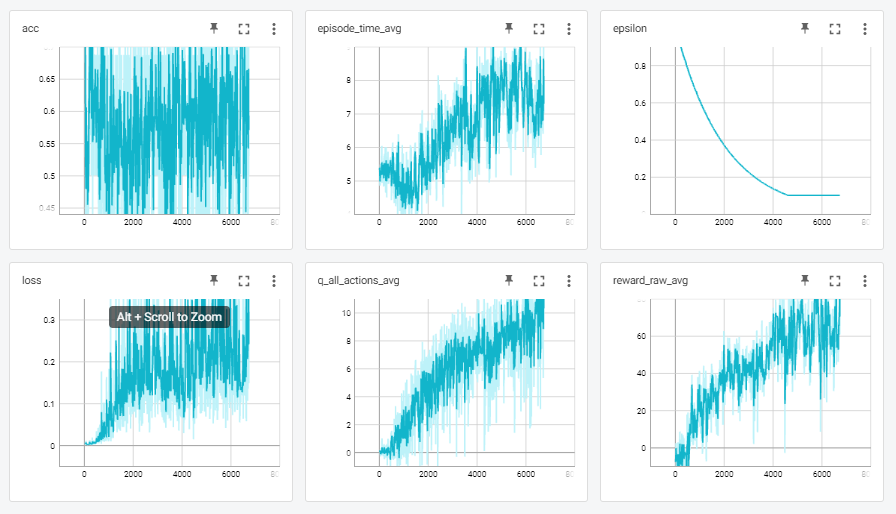
\includegraphics[width=1\linewidth]{images/tensorboard_bundaran_simpangempat_segmentasi_grayscale}
	\caption{Tensorboard pada Bundaran Simpang Empat dengan Segmentasi Grayscale}
	\label{fig:tensorboard_bundaran_simpangempat_segmentasi_grayscale}
\end{figure}

Dari hasil visualisasi training DQN pada Gambar \ref{fig:tensorboard_bundaran_simpangempat_segmentasi_grayscale}, dapat dilihat bahwa proses training algoritma DQN telah berjalan dengan baik. Hal itu dapat dilihat dari nilai akurasi, episode time, dan reward berkendara mobil otonom yang mengalami tren kenaikan seiring dengan berjalannya proses training.

\subsection{Training DQN pada Bundaran Simpang Empat dengan Segmentasi Lanjutan}
\label{sec:training_dqn_bundaran_simpangempat_segmentasi_hitam_putih}

\subsection{Training DQN pada Bundaran Tanpa Simpang dengan Segmentasi Lanjutan}
\label{sec:training_dqn_bundaran_nosimpang_segmentasi_hitam_putih}

\iffalse
Training algoritma DQN dengan
berlangsung selama 81 jam, 12 menit, dan 38 detik. Berikut adalah hasil visualisasi training algoritma DQN:

\begin{figure}[H] 
	\centering
	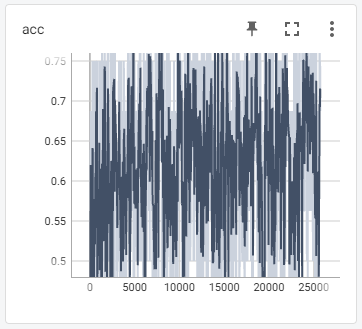
\includegraphics[width=.7\linewidth]{images/acc}
	\caption{Nilai akurasi}
	\label{fig:acc}
\end{figure}
\begin{figure}[H] 
	\centering
	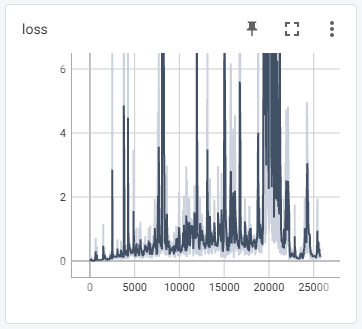
\includegraphics[width=.7\linewidth]{images/loss}
	\caption{Nilai loss}
	\label{fig:loss}
\end{figure}
\begin{figure}[H] 
	\centering
	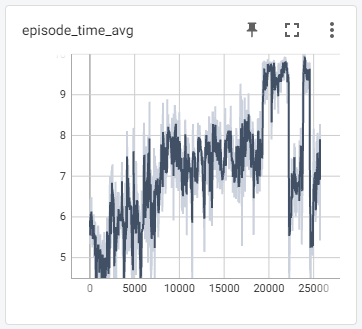
\includegraphics[width=.7\linewidth]{images/episode_time_avg}
	\caption{Rerata waktu episode}
	\label{fig:episode_time_avg}
\end{figure}
\begin{figure}[H] 
	\centering
	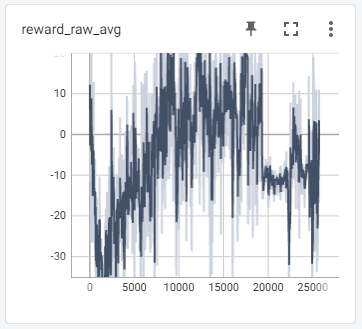
\includegraphics[width=.7\linewidth]{images/reward_raw_avg}
	\caption{Rerata nilai reward \textit{raw}}
	\label{fig:reward_raw_avg}
\end{figure}
\begin{figure}[H] 
	\centering
	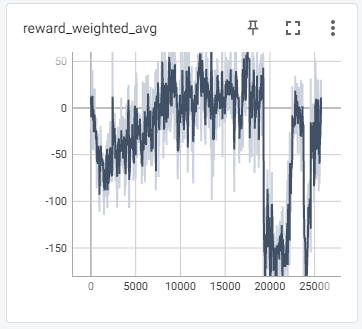
\includegraphics[width=.7\linewidth]{images/reward_weighted_avg}
	\caption{Rerata nilai reward \textit{weighted}}
	\label{fig:reward_weighted_avg}
\end{figure}
\begin{figure}[H] 
	\centering
	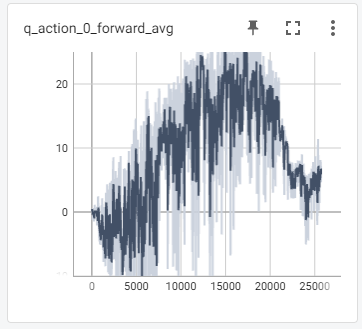
\includegraphics[width=.7\linewidth]{images/q_action_0_forward_avg}
	\caption{Nilai rerata q dari action forward}
	\label{fig:q_action_0_forward_avg}
\end{figure}
\begin{figure}[H] 
	\centering
	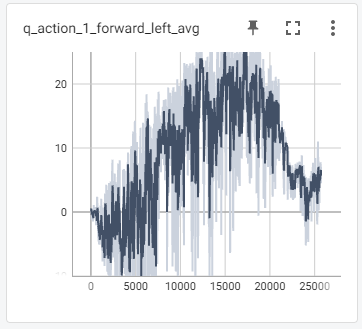
\includegraphics[width=.7\linewidth]{images/q_action_1_forward_left_avg}
	\caption{Nilai rerata q dari action forward left}
	\label{fig:q_action_1_forward_left_avg}
\end{figure}
\begin{figure}[H] 
	\centering
	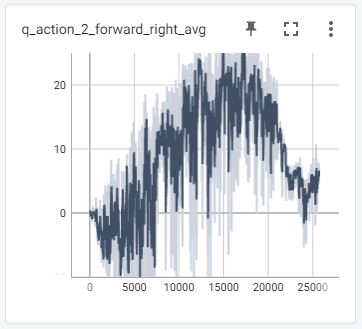
\includegraphics[width=.7\linewidth]{images/q_action_2_forward_right_avg}
	\caption{Nilai rerata q dari action forward right}
	\label{fig:q_action_2_forward_right_avg}
\end{figure}
\begin{figure}[H] 
	\centering
	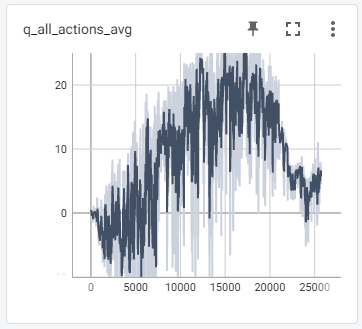
\includegraphics[width=.7\linewidth]{images/q_all_actions_avg}
	\caption{Nilai rerata q dari seluruh action}
	\label{fig:q_all_actions_avg}
\end{figure}

Dari hasil visualisasi training DQN diatas, dapat dilihat bahwa proses training algoritma DQN telah berjalan dengan baik. Hal itu dapat dilihat dari nilai akurasi, \textit{episode time}, dan \textit{reward} berkendara mobil otonom yang mengalami tren kenaikan seiring dengan berjalannya proses training.

\fi

\section{Pengujian Model DQN}
\label{sec:pengujian_model_dqn}

Pada bagian ini, akan dilakukan pengujian model hasil dari proses training DQN. Pengujian dilakukan saat lingkungan berkendara dalam kondisi normal.

\subsection{Pengujian Model DQN pada Bundaran Simpang Empat dengan Segmentasi Grayscale}
\label{sec:pengujian_dqn_bundaran_simpangempat_segmentasi_grayscale}

Setelah dilakukan tiga kali pengujian, didapatkan hasil seperti berikut:

% Please add the following required packages to your document preamble:
% \usepackage{graphicx}
\begin{table}[H]
	\resizebox{\columnwidth}{!}{%
		\begin{tabular}{|l|l|l|l|l|}
			\hline
			episode\_time & speed\_avg & angle\_deviation\_avg & distance\_deviation\_avg & reward\_avg \\ \hline
			24            & 40.2       & 17.3                  & 2.0                      & 0.32        \\ \hline
			25            & 40.1       & 20.8                  & 1.7                      & 0.28        \\ \hline
			16            & 38.8       & 16.6                  & 1.8                      & 0.32        \\ \hline
		\end{tabular}%
	}
	\caption{Hasil pengujian.}
	\label{tb:hasilpengujian}
\end{table}


\subsection{Pengujian Model DQN pada Bundaran Simpang Empat dengan Segmentasi Lanjutan}
\label{sec:pengujian_dqn_bundaran_simpangempat_segmentasi_hitam_putih}

\subsection{Pengujian Model DQN pada Bundaran Tanpa Simpang dengan Segmentasi Lanjutan}
\label{sec:pengujian_dqn_bundaran_nosimpang_segmentasi_hitam_putih}


\iffalse
\subsection{Hasil Setelah Learning 12 jam}
\label{sec:hasil_learning_12}
Setelah learning selama 12 jam, didapatkan model reinforcement yang sudah cukup memahami kehadiran bundaran di depan agent. Pada salah satu run simulasi Gambar \ref{fig:uji0}, didapatkan agent yang mampu bergerak lurus ke depan hingga mendekati bundaran, dan mampu melakukan manuver kanan lalu ke kiri lagi (dan arah kembali sejajar dengan arah pada saat start) agar tidak menyentuh bundaran. Meskipun pada akhirnya agent menyentuh object rumah pada ujung jalan.

\begin{figure}[H] 
	\centering
	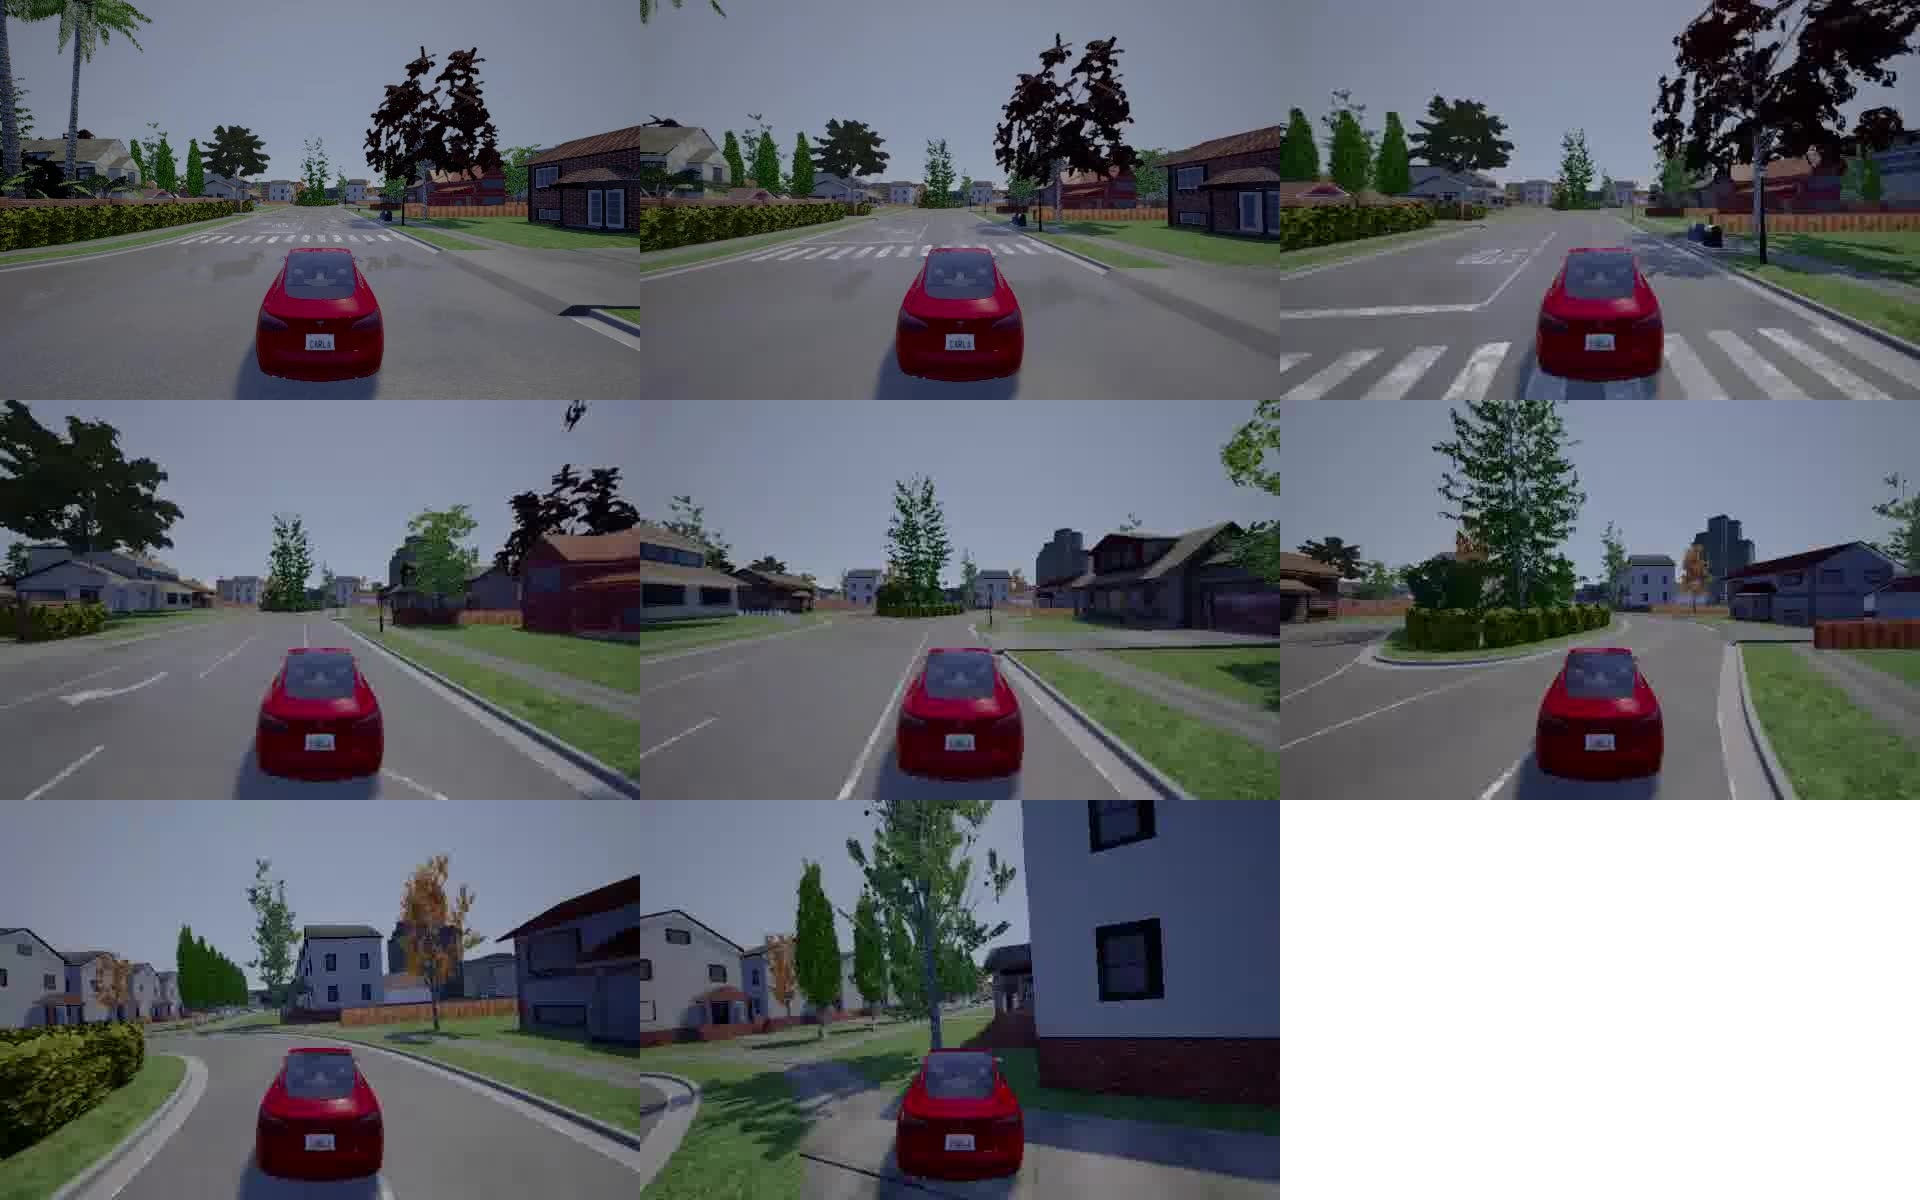
\includegraphics[width=1\linewidth]{images/uji0}
	\caption{Salah satu hasil simulasi uji. Jarak antar foto adalah 1.5 detik. Baca sekuen dari atas kiri ke kanan bawah.}
	\label{fig:uji0}
\end{figure}

\subsection{Hasil Setelah Learning 58 jam}
\label{sec:hasil_learning_12}
Setelah learning selama 58 jam, didapatkan model reinforcement yang sudah cukup memahami gerakan bahwa agent harus memutari bundaran agar mendapatkan award yang lebih besar. Pada salah satu run simulasi Gambar \ref{fig:uji1}., didapatkan agent yang mampu bergerak lurus ke depan hingga mendekati bundaran, dan mampu melakukan manuver kiri untuk menghindari bundaran, lalu melakukan manuver ke kanan mengitari bundaran dan tidak menyentuh bundaran. Meskipun pada akhirnya agent menyentuh object pagar setelah mengitari hampir 3/4 dari bundaran.
\begin{figure}[H] 
	\centering
	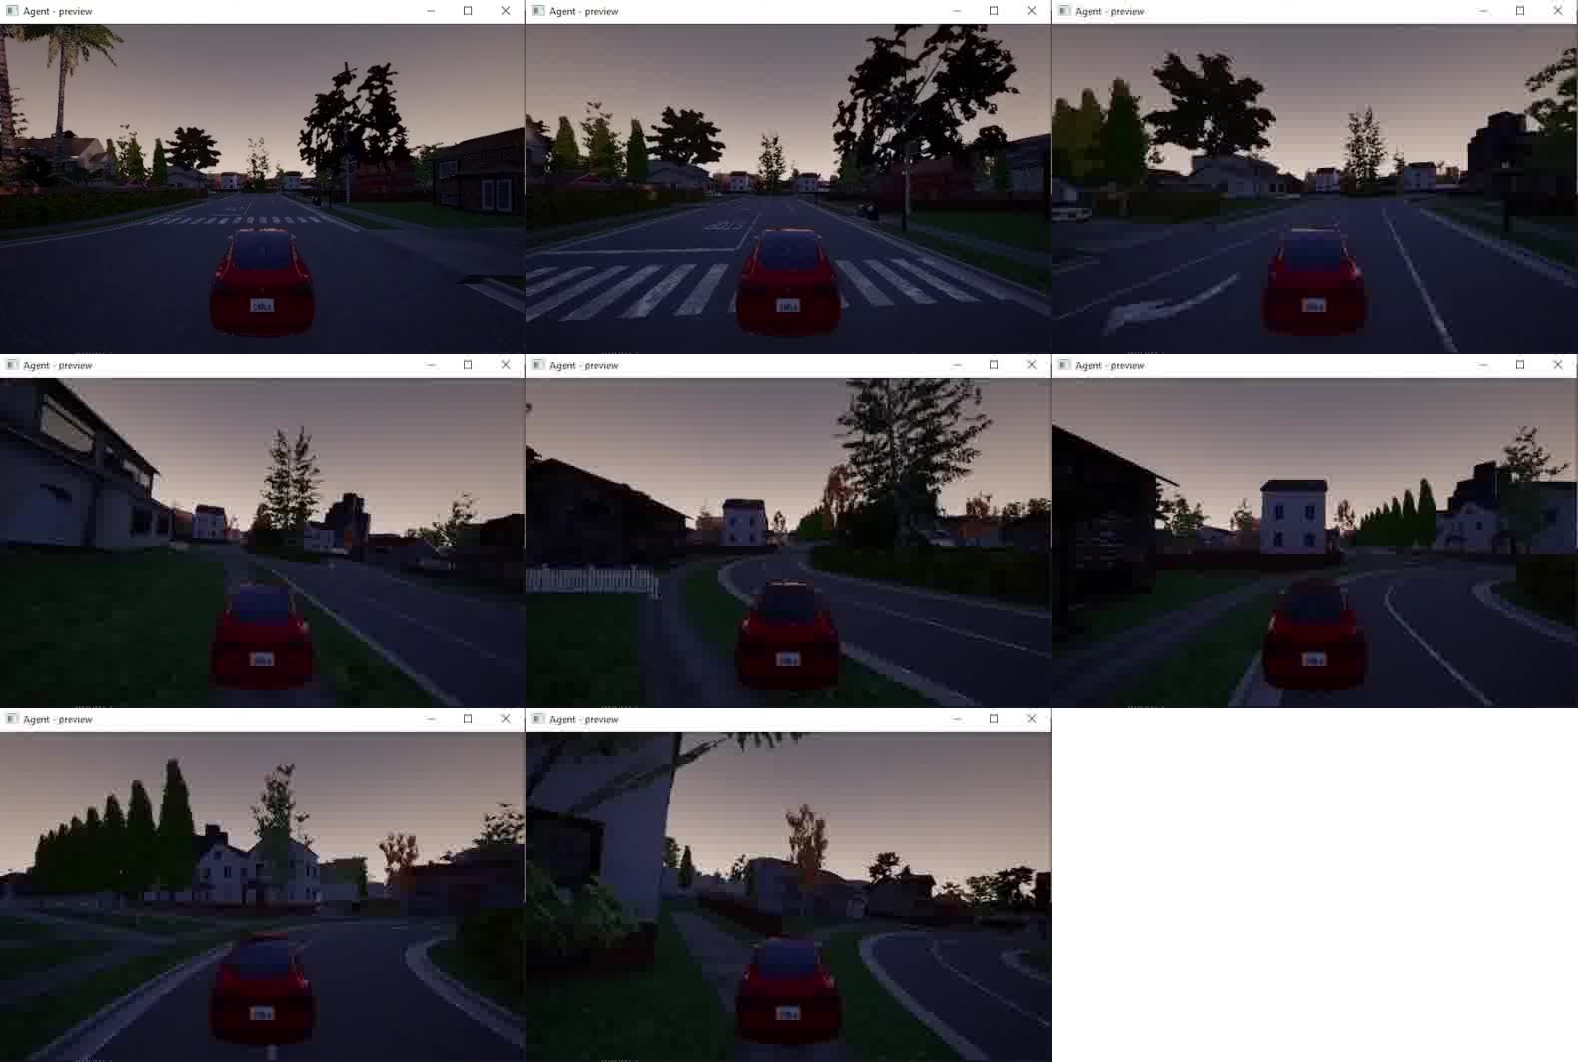
\includegraphics[width=1\linewidth]{images/uji1}
	\caption{Salah satu hasil simulasi uji. Jarak antar foto adalah 1.2 detik. Baca sekuen dari atas kiri ke kanan bawah.}
	\label{fig:uji1}
\end{figure}
\fi

  \cleardoublepage

  % Bab 5 penutup
  \chapter{PENUTUP}
\label{chap:penutup}

% Ubah bagian-bagian berikut dengan isi dari penutup

\section{Kesimpulan}
\label{sec:kesimpulan}

Dari perancangan dan pengujian sistem yang telah dilakukan, diperoleh beberapa kesimpulan sebagai berikut. 

\begin{enumerate}[nolistsep]

  \item Sistem perencanaan gerakan mobil otonom berbasis algoritma \textit{reinforcement learning} \textit{Deep Q Network} yang dirancang mampu melakukan akselerasi dan \textit{steer} yang mampu mengontrol mobil otonom dan melakukan manuver di bundaran dan/atau \textit{u-turn}.

  \item Penggunaan \textit{state } citra dengan segmentasi lanjutan; yaitu citra \textit{drivable }dan \textit{non-drivable} menghasilkan hasil yang lebih baik daripada segmentasi biasa dengan performa \textit{average\_episode\_length} 42.8\% lebih baik, \textit{average\_speed} 15.3\% lebih baik, dan \textit{average\_distance\_difference} 112.4\% lebih baik.

\end{enumerate}

\section{Saran}
\label{chap:saran}

Untuk pengembangan selanjutnya pada topik penelitian perencanaan gerakan mobil otonom dengan menggunakan algoritma DQN, terdapat beberapa saran yang diberikan, antara lain sebagai berikut:

\begin{enumerate}[nolistsep]

  \item Sensor yang digunakan untuk navigasi dari \textit{agent }menggunakan algoritma DQN dapat ditambah menjadi lebih banyak seperti GPS serta LIDAR, agar \textit{agent} dapat bertindak dengan parameter yang lebih lengkap.

  \item Proses training dapat dilakukan dengan waktu yang lebih panjang serta menggunakan mesin dengan tenaga komputasi yang lebih kuat agar didapatkan model yang konvergen.

  \iffalse
  \item Memperbaiki sistem award, dimana sebaiknya memikirkan sudut kendaraan terhadap pusat bundaran, serta jarak kendaraan terhadap bagian tengah jalan.

  \item Membuat tolak ukur metrik yang memadai untuk bagian pengujian model berupa plot riwayat gerakan kendaraan serta plot kecepatan kendaraan.
  \fi

\end{enumerate}

  \cleardoublepage

  % Daftar pustaka
  \renewcommand\bibname{DAFTAR PUSTAKA}
  \addcontentsline{toc}{chapter}{\bibname}
  \bibliographystyle{unsrtnat}
  \bibliography{pustaka/pustaka.bib}
  \cleardoublepage

  % Biografi penulis
  \begin{center}
  \Large
  \textbf{BIOGRAFI PENULIS}
\end{center}

\addcontentsline{toc}{chapter}{BIOGRAFI PENULIS}

\vspace{2ex}

\begin{wrapfigure}{L}{0.3\textwidth}
  \centering
  \vspace{-3ex}
  % Ubah file gambar berikut dengan file foto dari mahasiswa
  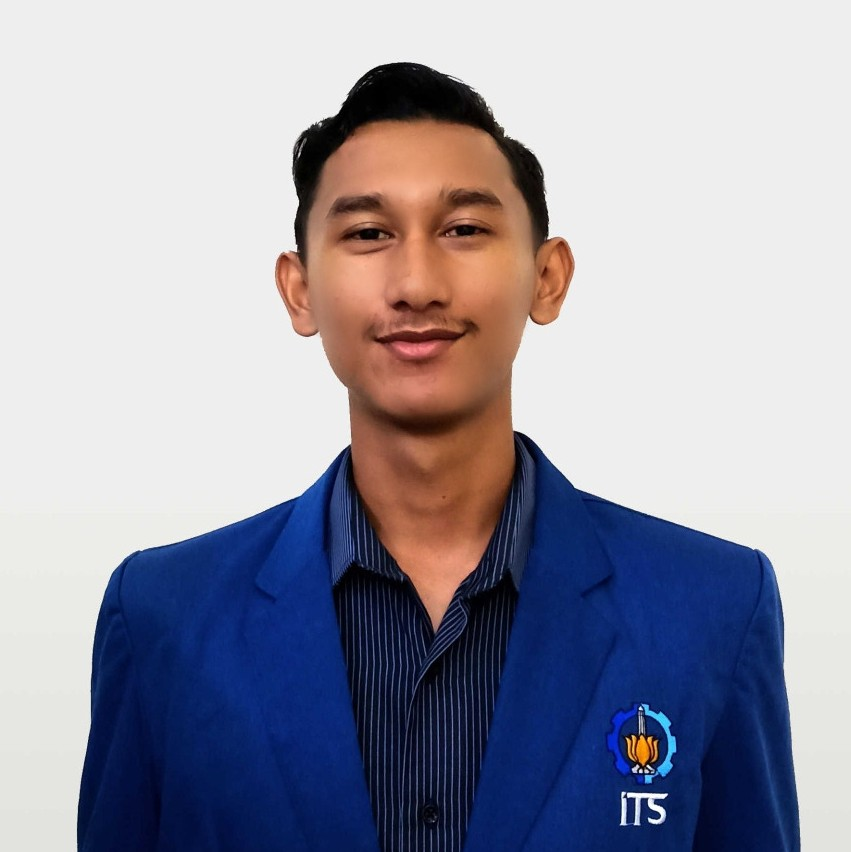
\includegraphics[width=0.3\textwidth]{images/roy.jpg}
  \vspace{-4ex}
\end{wrapfigure}

% Ubah kalimat berikut dengan biografi dari mahasiswa
Muhammad Roychan Meliaz, lahir pada 30 Mei 1999 di Kota Batam. Penulis telah menyelesaikan pendidikan formal di SDIT Darussalam 01 Batam (2005-2011), SMPN 03 Batam (2011-2014), dan SMAN 1 Batam (2014-2017). Pada tahun 2017 penulis melanjutkan studi S1 di Institut Teknologi Sepuluh Nopember (ITS) di Surabaya, dengan Departemen Teknik Komputer. Selama masa perkuliahan, penulis aktif mengikuti kegiatan organisasi dan kepanitiaan yang terdapat di kampus, seperti MAGE dan beberapa kegiatan lainnya. Penulis juga aktif sebagai asisten laboratorium di Lab B201 Telematika, serta menjadi bagian dari tim Kontes Robot ABU Indonesia (KRAI) ITS dan telah bertanding di Kontes Robot Indonesia. Di luar kampus, penulis juga aktif sebagai pengurus di Forum Daerah (Forda) Kerukunan Pelajar Mahasiswa Kepulauan Riau – Surabaya (KPMKR-Surabaya) yang menaungi para pelajar dan mahasiswa asal Provinsi Kepulauan Riau yang melanjutkan studi pendidikan di Kota Surabaya. Untuk mengubungi penulis, dapat melalui alamat email berikut roychan.meliaz@gmail.com. 



  \cleardoublepage

\end{document}
